% !TEX program = xelatex
% 2026 年高教社杯全国大学生数学建模竞赛 A 题
% 药材的烘干问题 —— 论文全文（单文件完整版）
% 由 摘要与总论.tex、问题一.tex、问题二三四.tex 合并而成

\documentclass[12pt,a4paper,fontset=none]{ctexart}

% 中文字体：显式指定，避免依赖系统字体集探测
\usepackage{xeCJK}
\setmainfont{Times New Roman}
\setsansfont{Arial}
\setmonofont{Menlo}
\setCJKmainfont{Songti SC}
\setCJKsansfont{Heiti SC}
\setCJKmonofont{Songti SC}

\usepackage{amsmath,amssymb,bm}
\usepackage{booktabs}
\usepackage{multirow}
\usepackage{array}
\usepackage{geometry}
\usepackage{caption}
\usepackage{graphicx}
\usepackage{xcolor}
\usepackage{listings}

% 代码清单样式：行号 + 细边框 + 语法高亮，中文字注释由 xeCJK-listings 处理
\lstset{
  basicstyle=\ttfamily\scriptsize,
  numbers=left,
  numberstyle=\tiny\color{black!45},
  numbersep=8pt,
  % 行号默认画在清单框左侧、伸进页边距里（实测越界约 0.6cm）。
  % 下面两项让清单整体右移、同时把框向左扩到行号外侧，
  % 使"框＋行号"的总宽度恰好等于正文宽度。
  xleftmargin=2.4em,
  framexleftmargin=2.4em,
  xrightmargin=0em,
  framexrightmargin=0em,
  frame=single,
  framesep=2pt,
  rulecolor=\color{black!35},
  breaklines=true,
  breakatwhitespace=false,
  columns=fullflexible,
  keepspaces=true,
  showstringspaces=false,
  tabsize=4,
  language=Python,
  keywordstyle=\color{blue!70!black},
  commentstyle=\color{green!45!black},
  stringstyle=\color{red!55!black},
  extendedchars=true,
  captionpos=b,
}

\geometry{left=2.2cm,right=2.2cm,top=2.6cm,bottom=2.4cm}
% 页码：格式规范要求"页码位于页脚中部，用阿拉伯数字从 1 开始连续编号"，
% 故不用带页眉的 headings 样式（页眉会把页码顶到右上角）。
\pagestyle{plain}
\captionsetup{font=small,labelsep=quad}
\linespread{1.00}
\allowdisplaybreaks
\setlength{\emergencystretch}{3em}

% 浮动体：允许每页容纳更多表格/插图，并压缩它们与正文之间的空白，
% 避免出现"两张表被顶到同一页、中间空出一大块"的版面。
\setcounter{topnumber}{3}
\setcounter{bottomnumber}{2}
\setcounter{totalnumber}{5}
\renewcommand{\topfraction}{0.92}
\renewcommand{\bottomfraction}{0.6}
\renewcommand{\textfraction}{0.07}
\renewcommand{\floatpagefraction}{0.8}
\setlength{\textfloatsep}{8pt plus 2pt minus 2pt}
\setlength{\floatsep}{8pt plus 2pt minus 2pt}
\setlength{\intextsep}{8pt plus 2pt minus 2pt}

\begin{document}


\begin{center}
  {\zihao{3}\bfseries 药材烘干过程的传热传质建模与数值仿真}
\end{center}

\vspace{0.5em}
\begin{center}
  {\zihao{4}\bfseries 摘\quad 要}
\end{center}

\noindent
针对圆柱形中药材的热风烘干，本文建立圆柱坐标系下一维径向的\textbf{耦合抛物型
偏微分方程组}（含变物性的能量方程与 Fick 型水分扩散方程），用节点中心有限
体积法离散、后向 Euler 全隐式推进、Picard 迭代处理非线性，四个问题共用同一
套求解内核，依次引入变物性、两阶段工况与干燥判据、移动边界与收缩，保证结论
之间自洽可比。本文的着力点不在求解本身，而在题面未给定的闭合关系与结果
可信度的分层检验：\textbf{输入与闭合是否可信、数值解是否可信、模型假设是否
可信}。

\textbf{数据层面}，附件 1 的残差为高频交替型抖动、无异常点，故不作平滑，
并在线性插值、保单调三次 Hermite 插值（PCHIP）与三次样条中保留不产生
过冲的分段线性插值；附件 2 的半径序列则用 PCHIP，获得不过冲、$C^1$ 连续
的收缩几何。
同时指出：仅凭空气侧激励无法反演换热系数 $h$ 与传质系数 $h_m$，故用灵敏度
分析替代参数标定，并据测量噪声确定温度结果只有 3 位有效数字。尺度分析给出
物理主线：$\alpha=1.689\times10^{-7}$\,m$^2$/s 是
$D(C_0)=4.938\times10^{-9}$\,m$^2$/s 的 $34$ 倍，1800\,s 内热扩散长度
$17.4$\,mm 已接近半径、而水分扩散长度仅 $2.98$\,mm。

\textbf{数值层面}，本文区分\textbf{报告网格与求解网格}：把题面 $0.1$\,cm 的
输出网格直接当作求解网格，会因网格误差把烘干时长低估 $1.6\%$；空间离散一阶
收敛、时间离散误差仅 $0.2\%$。更重要的是，水分方程口径带来的 $+6.3\%$ 差异
在 $N=20\sim400$、$\Delta t=2\sim120$\,s 共 20 组参数下保持不变，据此判定它属
\textbf{模型层面}而非离散层面，不能靠加密网格消除，也不应被误读为数值误差。

\textbf{模型结构层面}，由恒等式 $\rho=\rho_d(1+C)$ 证明“斜率等于截距”等价于
“体积不变”，把题面经验式的 $b<a$ 从“数据矛盾”翻译为\textbf{收缩的定量标志}，
并给出以斜率截距比 $r=b/a$ 为单参数的先验判据：$5\%$ 半径容差下预热窗口阈值
$r^\ast=0.164$，附录 3 通过（线收缩 $4.57\%$）、附录 4 已越界（$5.68\%$）；
全程窗口阈值升到 $0.838$，两套物性都必须在问题四计入收缩。同一层面还判定
两处题面未言明的闭合关系：按题给传质关系构造蒸发潜热通量会把表面温度压至
$6.1\,^\circ$C，低于由空气状态算得的湿球温度 $34.7\,^\circ$C，出现非物理解，
说明题面参数体系对应忽略汽化潜热的简化；而密度经验式与实测收缩半径隐含的
干物质质量并不守恒（问题三 $+116\%$、问题四 $-10.9\%$），本文如实报告并把结果
定位为“题面给定数据体系下的自洽解”。

\textbf{四个问题的结果}：问题一中 $D$ 只依赖 $C$、其余物性为常数，热方程与
水分方程\textbf{完全解耦}，1800\,s 时中心温度 $33.5765\,^\circ$C、表面
$36.7863\,^\circ$C，中心含水率始终 $2.5500$\,kg/kg、表面降至 $1.5103$\,kg/kg，
水分变化限于最外侧 $3\sim5$\,mm；若退化为均温均湿的\textbf{集总参数模型
（单个常微分方程）}，脱水只需约 $11.2$\,h，仅为分布参数结果的 $19.5\%$，
可见径向梯度是决定烘干时长的本体。问题二中物性随 $C$、$T$ 变化，两方程转为
强耦合，3\,h 内基本达到烘房温度（径向温差 $0.12\,^\circ$C）；问题三中
“各处含水率低于 $0.15$\,kg/kg”等价于中心达标，得
\textbf{烘干时长 57.42\,h（2.392 天）}，其中最后 $21$\,h 只换来 $0.036$\,kg/kg
的下降，末段由扩散系数只有芯部 $1/256$ 的干壳控制；问题四采用实测收缩半径与
贴体坐标 $\xi=r/R(t)$，因 $\xi$ 同时是材料坐标，骨架对流项与坐标变换项
\textbf{精确抵消}，水分方程与问题二、三同口径，得
\textbf{烘干时长 51.08\,h（2.128 天）}；同物性、同口径下固定半径需 $129.79$\,h，
即\textbf{忽略收缩会把烘干时长高估为 2.54 倍（154\%）}。

全部结论经过网格、时间步、界面取法、水分口径、参数灵敏度与干物质守恒六类
自检，误差来源可排序、结论可复核：$D$ 的不确定度（$\pm20\%$ 对应
$48.9\sim70.0$\,h）$>$ 水分方程口径（$+6.3\%/-15.6\%$）$>$ 界面取法
（$N=200$ 上 $2.7\%$）$>$ 题面输出网格 $N=20$（$1.6\%$）$>$ 端面效应
（不超过 $1.1\%$）$>$ 时间步（$0.2\%$）$>$ 表面换热系数（$0.03\%$）；
本文采用的 $N=200$ 网格误差仅 $0.07\%$。

\vspace{1em}
\noindent\textbf{关键词}：
抛物型偏微分方程组；常微分方程；有限体积法；数值模拟；移动边界与收缩；参数灵敏度分析

\section{问题提出}

中药材烘干以热风烘干为主\cite{ref-pan}，分预热平衡与恒温干燥两个阶段；工艺参数选取
不当会造成效率低、能耗高、品质不稳等问题，而传统试验优化成本高、周期长，
可以借助数理分析与数值仿真更快的获得干燥规律。

某圆柱形中药材长 25\,cm、半径 2\,cm，初始温度 28\,$^\circ$C、
初始干基含水率 2.55\,kg/kg。已知烘房空气的温度与水分浓度、烘干过程中药材半径的变化，
给定问题一的物性参数，给出问题二、三、四的经验公式。需要解决：

\begin{enumerate}
  \item 建立预热平衡阶段药材温度与水分浓度变化的数学模型，
        给出 1800\,s 内按指定时空格点采样的结果；
  \item 建立整个烘干过程（预热平衡 $+$ 恒温干燥）的数学模型，
        给出 3\,h 内的结果；
  \item 按各处含水率低于 0.15\,kg/kg的要求确定烘干所需时间；
  \item 考虑药材因失水发生的尺寸和$\rho$变化，重新确定烘干时长。
\end{enumerate}

\section{问题分析}

四个问题本质是求解同一个物理过程的不同层面，逻辑关系见表 \ref{tab:overview}：

\begin{table}[htbp]
  \centering
  \caption{四个问题的逻辑关系}
  \label{tab:overview}
  \small
  \begin{tabular}{lllll}
    \toprule
    问题 & 物性来源 & 时间跨度 & 核心要求 & 解法 \\
    \midrule
    一 & 附录 2（恒定）        & 30 min  & 预热平衡 & 热、质方程解耦 \\
    二 & 附录 3（随 $C$、$T$变化） & 0-3 h & 全流程耦合 & 强耦合，需联立迭代 \\
    三 & 同问题 2             & 2--3 天 & 烘干时长 & 反求达标时刻 \\
    四 & 附录 4（随 $C$、$T$变化） & 2--3 天 & $\rho$和尺寸变化 & 动边界，需坐标变换 \\
    \bottomrule
  \end{tabular}
\end{table}

问题的物理内核是\textbf{含湿多孔介质内的耦合传热传质}：热量由表面向内传导、
水分由内向外迁移并在表面被空气带走，两者通过随含水率与温度变化的物性
相互影响。三个量级分析决定了建模方向：长径比与端面占比说明可退化为一维
径向问题；热扩散率与水分扩散系数相差数十倍，说明两场时间尺度不同、预热
阶段以达热平衡为主；两个 Biot 数均处于中值区间，说明不能作集总参数近似。

本文的技术路线是\textbf{同一个模型的四次升级}:
共同基础是圆柱坐标系下的一维径向耦合传热传质方程、节点中心有限体积、
后向 Euler 全隐式推进与追赶法求解；在此基础上依次引入
变物性（问题二）$\to$ 两阶段工况与干燥判据（问题三）
$\to$ 移动边界与变化的$\rho$（问题四）。四个问题具有一套共同的基础，
    保证了结论之间的自洽与可比。

\section{模型假设}

全文假设分为介质与几何、物性与边界、闭合关系与数据处理三类，共
(A1)--(A10) 条，逐条列于下；每条均注明依据或对应的检验小节。

\begin{enumerate}
  \item[(A1)] \textbf{介质与局部热平衡}：药材视为均质、各向同性的含湿
        多孔介质；局部热平衡，不区分两相温度；固相体积分数允许随干燥收缩
        而变化，但固相自身不可压缩、干物质质量守恒。
  \item[(A2)] \textbf{降维}：忽略轴向输运，问题简化为一维径向轴对称。
        依据是长度半径比 $L/R=12.5$（长径比 $L/(2R)=6.25$）、
        两端面总面积仅占侧面积的 $R/L=8\%$
        （误差分析见第 \ref{sec:radial} 节）。
  \item[(A3)] \textbf{热源与辐射}：只考虑对流换热与对流传质\cite{ref-wang}；
        烘房空气温度、湿度与流速在药材表面均匀分布，$h$ 与 $h_m$ 沿周向和轴向不变。
  \item[(A4)] \textbf{几何}：问题一至三取固定半径 $R=2$\,cm，问题四按附件 2 的实测
        $R(t)$ 收缩。误差分析见第
        \ref{sec:shrink-criterion} 节。
  \item[(A5)] \textbf{物性}：按各问对应的附录取值；
        经验式只在实验区间 $C\in[0,2.55]$ 内使用，不作外推。
  \item[(A6)] \textbf{界面系数}：$h$ 与 $h_m$ 题面未给出，统一沿用附录 2 的
        $h=25$\,W/(m$^2\cdot$K)、$h_m=8\times10^{-7}$\,m/s。其可信度由灵敏度
        分析回答（第 \ref{sec:sensitivity} 节）。
  \item[(A7)] \textbf{汽化潜热}：忽略蒸发吸热对表面能量平衡的贡献。
        依据与能量收支核算见第 \ref{sec:closure} 节。
  \item[(A8)] \textbf{水分输运}：问题一至三用 Fick 型扩散描述\cite{ref-crank}，
        表面为第三类边界条件 $-D\left.\partial_rC\right|_{r=R}
        =h_m(C_s-C_\infty)$，且干基密度在方程两侧约去（第
        \ref{sec:rho} 节）；问题四考虑收缩，几何改用贴体坐标下的动区域，
        但水分方程仍是经典 Fick 口径——在材料坐标下对流项与坐标变换项
        精确抵消（式 \eqref{eq:p4-cancel}），故 \eqref{eq:p4-mass} 与
        问题二的 \eqref{eq:p2-mass} 形式相同，只多出度量因子 $R(t)^2$。
  \item[(A9)] \textbf{边界数据}：附件 1 的烘房温湿度实测序列
        \textbf{不作平滑、不作差分、不剔除观测点}，
        依据与量化影响见第 \ref{sec:preproc} 节。
  \item[(A10)] \textbf{收缩速率}：附件 2 的半径序列改用保单调三次 Hermite
        插值（PCHIP），理由见第
        \ref{sec:preproc} 节。
\end{enumerate}

\section{符号说明}

下表汇总全文通用符号及其含义与单位，正文中不再重复说明。

\begin{center}
\begin{minipage}{\textwidth}
  \centering
  \small
  \textbf{主要符号}\\[4pt]
  \begin{tabular}{cll}
    \toprule
    符号 & 含义 & 单位 \\
    \midrule
    $r,\ t$            & 径向坐标、时间              & m, s \\
    $T,\ C$            & 药材温度、干基含水率        & $^\circ$C, kg/kg \\
    $R,\ L$            & 药材半径、长度              & m \\
    $\xi$              & 贴体坐标 $\xi=r/R(t)$       & --- \\
    $T_\infty,C_\infty$ & 烘房空气温度、水分浓度     & $^\circ$C, kg/kg \\
    $\rho,\ c_p,\ k$   & 密度、比热容、热传导系数    & kg/m$^3$, J/(kg$\cdot$K), W/(m$\cdot$K) \\
    $D$                & 水分扩散系数                & m$^2$/s \\
    $h,\ h_m$          & 对流换热、传质系数          & W/(m$^2\cdot$K), m/s \\
    $\alpha$           & 热扩散率                    & m$^2$/s \\
    $Bi,\ Bi_m$        & 传热、传质 Biot 数          & --- \\
    $r=b/a$            & 密度经验式的斜率截距比      & --- \\
    $\beta,\ \varepsilon_r,\ \varepsilon_w$
                       & 端点收缩系数、径向线应变、水体积分数 & --- \\
    $\lambda,\ \mu$    & 径向、轴向特征值            & 1/m \\
    $w_i$              & 有限体积控制体权重          & m$^2$ \\
    $t_{\mathrm{dry}}$ & 烘干时长                    & s \\
    \bottomrule
  \end{tabular}
\end{minipage}
\end{center}

\section{数据预处理与物性数据的可容许性检验}
\label{sec:preproc}

本节先作数据质量诊断，再说明\textbf{附件 1 不作平滑、不作高阶插值、
不作差分，而附件 2 作保单调插值}的原因，并量化这些选择的影响。

\subsection{附件 1 的数据质量诊断}

附件 1 共 241 点、间隔 60\,s、覆盖 $0\sim14400$\,s。用无相位滞后的局部二次
多项式分离趋势后，残差统计见表 \ref{tab:noise}：滞后 1 自相关为负，说明它是
传感器噪声与控温往复调节造成的\textbf{高频交替型}抖动，而非真实物理起伏；
最大残差仅为标准差的 2.3 倍，\emph{不存在需要判别与剔除的异常点}；序列
\textbf{无缺失、无负值，温度全局最低点即 $t=0$ 的 $28.0000\,^\circ$C}。
因此附件 1 \emph{不需要}通常意义上的清洗。

\subsection{附件 1 的预处理：不作平滑、保留线性插值、不作差分}

第一条结论是\textbf{不作平滑}。
表 \ref{tab:smooth} 给出四种处理方式对问题一结果的影响
（均取 $N=400$、$\Delta t=1$\,s）其中 3 点滑动平均与 5 点
Savitzky--Golay 的偏差与边界噪声不可消除的涨落同量级、物理上不可区分，而 15 点窗口的
$0.055\,^\circ$C 明显超出该量级，恰印证上述判断。平滑既不改变结论、又要
额外引入一个可调参数，故本文不作平滑。

第二条结论是\textbf{保留 60\,s 分段线性插值}。各种插值都严格通过观测点，
差别只在两点之间（表 \ref{tab:interp}），并且用现有数据无法判定哪种插值更准；而自然三次
样条会把交替型噪声插出观测中并不存在的极值，产生 $0.080\,^\circ$C 的过冲，
把烘房单调升温插成局部降温，属非物理结果。该差别虽在物理上可忽略，却大于
四位小数的舍入阈值 $5\times10^{-5}$，会使\textbf{温度表中约 $87\%$ 的格子
第 4 位小数随插值方式改变}，故必须锁定一种口径。本文锁定分段线性插值：
无参数、无过冲、保单调，且对观测点不作改动。

第三条结论是\textbf{不用差分估计变化率}。温度的相邻差分标准差为
$0.245\,^\circ$C，除以 60\,s 得 $0.0041\,^\circ$C/s 的伪梯度，而问题一所在的
$0\sim1800$\,s 真实升温速率（线性拟合）为 $0.0075\,^\circ$C/s，
\textbf{信噪比仅约 $2:1$}；差分把噪声放大 $1/\Delta t$ 倍，在这份数据上
不可用。需要变化率时必须像附件 2 那样，用保形插值的解析导数给出。

\subsection{恒温干燥段的外推依据}

附件 1 只覆盖 $0\sim14400$\,s（4\,h），而整个烘干过程长达约 57\,h，故
$t>14400$\,s 的边界条件必须外推。本文取常值 $T_\infty=50\,^\circ$C、
$C_\infty=0.05$\,kg/kg，依据来自数据本身：末 1\,h 温度的线性拟合斜率仅
$+0.003\,^\circ$C/h，末 10 个采样点在 $49.76\sim50.23\,^\circ$C 之间围绕
50\,$^\circ$C 抖动，水分浓度稳定在 $0.0498\sim0.0502$\,kg/kg，末 1\,h 平均值
分别为 $49.9989\,^\circ$C 与 $0.04999$\,kg/kg。可见烘房已进入恒温恒湿状态。

\subsection{附件 2 的预处理：保单调三次 Hermite 插值}

附件 2 共 145 点、间隔 1800\,s，半径由 2.000\,cm 单调收缩至 1.198\,cm。
半径以两种方式进入模型：一是收缩域中的度量因子 $1/R^2$ 与表面边界条件中的
$R$，二是第 \ref{sec:p11-crosscheck} 节反演收缩速率、判断“收缩何时完成”
所需的 $\dot R$。若直接对实测序列作差分，相邻差分的信噪比只有 $2:1$，
噪声会被放大 $1/\Delta t$ 倍；若用分段线性插值，$R$ 的斜率在节点处跳变，
会使进入扩散算子与边界条件的几何量出现阶梯。因此采用 Fritsch--Carlson\cite{ref-fc}
构造的保单调三次 Hermite 插值（PCHIP），它既保证
$C^1$ 连续，又保持数据单调、不产生过冲；数值检验表明插值后 $R(t)$ 单调递减、
$\dot R\le0$ 恒成立（三次样条在该序列上会出现过冲，故不采用）。

\subsection{参数不可反演与温度结果的有效位}
\label{sec:identify}

附件 1 是实测数据，但是无法用它反求表面换热系数 $h$ 与对流传质
系数 $h_m$。\textbf{这在本题中做不到}。附件 1 记录的是烘房空气状态，在模型中
是\emph{边界激励}；而 $h$、$h_m$ 出现在表面通量条件
$-k\,\partial_rT|_{r=R}=h(T_s-T_\infty)$ 中，要定出它必须同时知道\emph{通量}
与\emph{驱动势}，而附件 1 只给出驱动势的空气侧，药材侧的表面温度、表面
含水率与通量本身全部未知，属一个方程含两个未知量的不定方程问题。换言之，
把 $h$ 改为任意值，附件 1 的 241 个数据一个都不变，\emph{参数完全不可辨识}。
附件 2 的 $R(t)$ 虽是唯一的药材侧实测响应，但收缩并不等于失水（还包含结构
塌陷），且 $h_m$ 与扩散系数 $D$ 高度相关、无法分离，故单独用 $R(t)$ 反演
$h_m$ 同样不可靠。

本题的正问题参数由附录 2 直接给定：$h=25$\,W/(m$^2\cdot$K)、
$h_m=8\times10^{-7}$\,m/s，无需反演；既然二者是"给定值"而非"标定值"，
正确的补救手段是\textbf{灵敏度分析}——四个问题的结论对二者均不敏感
（第 \ref{sec:sensitivity} 节）。由此也确定了温度结果的有效位：边界噪声给
输出带来的不可消除不确定度约为 $0.02\,^\circ$C，故表 \ref{tab:p1-T}、
表 \ref{tab:p2-T} 中温度值的\textbf{第 4 位小数不具物理意义、有效位为 3 位}，
本文仍按题目要求保留四位小数，但末位仅用于满足格式规范；相比之下水分浓度场
的四位小数对边界数据处理方式完全不敏感（表 \ref{tab:smooth}、
\ref{tab:interp}），是可靠的有效数字。

\subsection{物性关联式的自洽性检验与守恒口径}
\label{sec:rho}
\label{sec:closure}

附录给出的物性经验式（$\rho$、$c_p$、$k$）与 $D(C,T)$ 是后续模型的数据基础。
其中体积密度 $\rho=a+bC$ 容易引起误解：附录 3 中 $a=650,\ b=128$，
附录 4 中 $a=760,\ b=90$，均有 $b<a$；若把 $\rho=\rho_d(1+C)$ 中的
$\rho_d$ 视为常数，似乎会得到``斜率应等于截距''，进而怀疑题面经验式不自洽。
实际上 $\rho_d$ 是以当前湿物料总体积为基准的表观干物质密度，只要干燥过程中
体积发生变化，它就不是常数。

本节只回答两个基础问题：\textbf{题面物性式是否具有物理可容许性，以及 $\rho$
应如何进入守恒方程}；至于如何由 $\rho=a+bC$ 提取收缩信息、建立``何时可以忽略
收缩''的先验判据并量化其对烘干时长的影响，统一放在第 11 节讨论，
以避免重复推导并突出该判据的独立性。推导与数值旁证统一放在
附录 \ref{app:rho}，主文只保留三条结论。

\begin{enumerate}
  \item \textbf{题面密度式并不自相矛盾，它隐含了干燥收缩。}
        由恒等式 $\rho=\rho_d(1+C)$（其中 $\rho_d=m_d/V$ 以当前总体积为
        基准）可知，``斜率等于截距''只在总体积不变时才成立；题面两组
        经验式均满足 $b<a$，恰好说明随 $C$ 降低、单位干物质所占总体积
        减小，与干燥收缩的物理图像一致。附录 \ref{app:rho} 另用三相体积
        分数与 $c_p$、$k$ 的混合律极限作了旁证。
  \item \textbf{$\rho$ 不直接写入问题二、三的水分方程。}这两问采用固定
        几何的经典 Fick 口径（不显式描述骨架运动），干料密度在方程两侧
        约去；把题面 $\rho(C)$ 直接写回水分累积项会混合两套闭合假设并
        导致干物质守恒失配。作为口径敏感性检验，该写法使问题三烘干时长
        系统性延长 $6.3\%$（表 \ref{tab:clos}）。
  \item \textbf{$\rho$ 仍按经验物性进入能量方程}，与 $c_p(C)$ 共同构成
        体积热容：
        \begin{equation}
          \rho(C)c_p(C)\frac{\partial T}{\partial t}
          =\frac{1}{r}\frac{\partial}{\partial r}
          \left(rk(C)\frac{\partial T}{\partial r}\right).
          \label{eq:energy-rho}
        \end{equation}
        因此``$\rho$ 不进入水分扩散方程''并不意味着忽略题面密度数据，
        而是\textbf{质量守恒与能量守恒中 $\rho$ 的物理角色不同}。
\end{enumerate}

蒸发潜热属于同一类口径问题：完整表面能量平衡应含 $-L_vj_w$ 项，但按题给
传质系数计入后表面温度会被压到湿球温度以下、与物理不相容\cite{ref-wang}，故本文按假设 A7
忽略汽化潜热；能量收支核算见附录 \ref{app:rho}。

\begin{figure}[htbp]
  \centering
  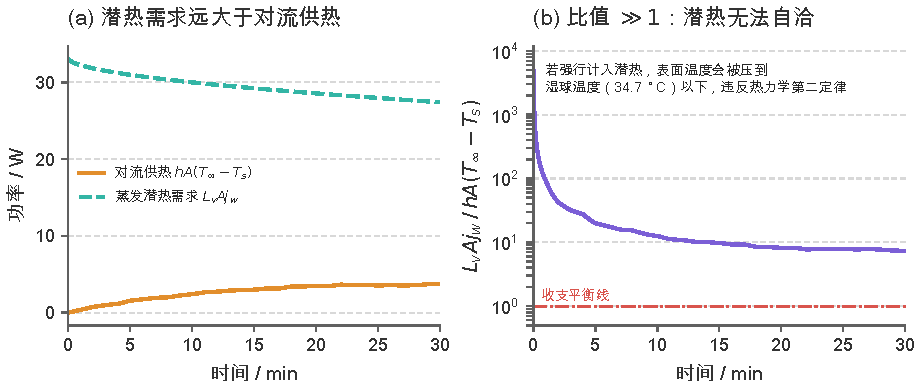
\includegraphics[width=\textwidth]{figs/d32_energy.pdf}
  \caption{蒸发潜热项的一致性检验：按题给 $h_m$ 估算的潜热需求远大于
    对流供热能力，比值全程大于 $1$，强行计入会把表面温度压到湿球温度
    以下，故题面参数体系对应忽略该项的简化（定量推导见附录
    \ref{app:rho}）。}
  \label{fig:energy}
\end{figure}

\section{问题一：预热平衡阶段药材温度与水分浓度模型}

\subsection{问题分析}

热风烘干过程中，烘房空气通过对流把热量传给药材表面，热量再向内部传导；
同时药材表层水分向空气迁移，形成由内向外的水分浓度梯度。预热平衡阶段的
任务是刻画药材内部温度场 $T(r,t)$ 与水分浓度场 $C(r,t)$ 随时间和径向位置
的演化规律。

题目给出的药材为圆柱体，长 $L=25$\,cm、半径 $R=2$\,cm，长径比为 $6.25$，
两端面面积仅占侧面积的 $8\%$，轴向输运可忽略，故可将问题降维为
\emph{一维径向轴对称}问题，$r\in[0,R]$。初始时刻药材温度 $T_0=28\,^\circ$C、
干基含水率 $C_0=2.55$\,kg/kg，烘房空气状态 $T_\infty(t)$、$C_\infty(t)$
由附件 1 给出，参数取自附录 2。

模型形态由三个量决定。由附录 2 的物性可得热扩散率
\[
  \alpha=\frac{k}{\rho c_p}=\frac{0.36}{820\times2600}
  =1.689\times10^{-7}\ \mathrm{m^2/s},
\]
而初始含水率下的水分扩散系数为
\[
  D(C_0)=7\times10^{-9}e^{-0.89/2.55}=4.938\times10^{-9}\ \mathrm{m^2/s},
\]
两者相差 $34$ 倍。在 $1800$\,s 内，热扩散特征长度
$\sqrt{\alpha t}=17.4$\,mm 已接近半径 $20$\,mm，而水分扩散特征长度
$\sqrt{Dt}=2.98$\,mm 还不足半径的 $1/6$。这说明：\textbf{30 分钟内热量已在
整个截面上基本重新分布，而含水率仅在表层发生变化}。这恰好是预热平衡
阶段的意义所在。

另外，换热与传质的 Biot 数分别为 $Bi=hR/k=1.389$ 与
$Bi_m=h_mR/D(C_0)=3.24$，意味着内部导热/扩散阻力与表面
对流阻力都不能被忽略，不能采用集总参数近似，必须给出沿半径的分布。

\subsection{模型假设与符号说明}

本章符号沿用第 4 节符号表。

本章沿用第 3 节的全局假设 (A1)--(A10)，不再引入新的简化。需要强调的是，
问题一的物性按附录 2 取\textbf{常数}，且水分扩散系数只依赖含水率
（$D=D(C)$，不含温度），这一条是后文"热--质解耦"结论的物理前提；
该结论在问题二起不再成立。

\subsection{模型建立}

\subsubsection{控制方程}

在圆柱坐标下，取控制体
$2\pi r\,\mathrm{d}r\,\mathrm{d}z$ 作能量与质量的守恒分析。热量守恒给出：
\begin{equation}
  \rho c_p\frac{\partial T}{\partial t}
  =\frac{1}{r}\frac{\partial}{\partial r}
   \left(k\,r\frac{\partial T}{\partial r}\right),
  \label{eq:p1-heat}
\end{equation}
水分守恒给出：

\begin{equation}
  \frac{\partial C}{\partial t}
  =\frac{1}{r}\frac{\partial}{\partial r}
   \left(D(C)\,r\frac{\partial C}{\partial r}\right).
  \label{eq:p1-mass}
\end{equation}
说明：由于式 \eqref{eq:p1-mass} 中 $\rho$ 为常数，已在等式两侧约去。
该建模选择在 §\ref{sec:closure} 中专门说明。

\subsubsection{定解条件}

初始条件为均匀场
\begin{equation}
  T(r,0)=T_0=28\,^\circ\mathrm{C},\qquad
  C(r,0)=C_0=2.55\ \mathrm{kg/kg}.
  \label{eq:p1-ic}
\end{equation}

中心 $r=0$ 处由对称性给出第二类齐次边界条件
\begin{equation}
  \left.\frac{\partial T}{\partial r}\right|_{r=0}=0,\qquad
  \left.\frac{\partial C}{\partial r}\right|_{r=0}=0 .
  \label{eq:p1-center}
\end{equation}

表面 $r=R$ 处为第三类边界条件，即对流换热与对流传质
\begin{equation}
  -k\left.\frac{\partial T}{\partial r}\right|_{r=R}
  =h\left(T_s-T_\infty(t)\right),
  \label{eq:p1-bc-heat}
\end{equation}
\begin{equation}
  -D\left.\frac{\partial C}{\partial r}\right|_{r=R}
  =h_m\left(C_s-C_\infty(t)\right),
  \label{eq:p1-bc-mass}
\end{equation}
其中 $T_s=T(R,t)$、$C_s=C(R,t)$。附件 1 只覆盖 $0\sim14400$\,s，
本问题求解区间为 $0\sim1800$\,s，全部落在附件范围内，
$T_\infty(t)$ 与 $C_\infty(t)$ 由实测数据线性插值得到。

\subsubsection{物性关系}

由附录 2，
\begin{equation}
  \rho=820\ \mathrm{kg/m^3},\quad
  c_p=2600\ \mathrm{J/(kg\cdot K)},\quad
  k=0.36\ \mathrm{W/(m\cdot K)},
\end{equation}
\begin{equation}
  h=25\ \mathrm{W/(m^2\cdot K)},\quad
  h_m=8\times10^{-7}\ \mathrm{m/s},
\end{equation}
\begin{equation}
  D(C)=7\times10^{-9}e^{-0.89/C}\quad(\mathrm{m^2/s}).
  \label{eq:p1-D}
\end{equation}
式 \eqref{eq:p1-D} 的指数为负：含水率越低扩散越慢。$C$ 由 $2.55$ 降到
$1.51$ 时，$D$ 由 $4.938\times10^{-9}$ 降至 $3.883\times10^{-9}$\,m$^2$/s
（降幅 $21\%$）；若继续干燥到 $C=0.15$，$D$ 将降至
$1.855\times10^{-11}$\,m$^2$/s，跨越两个数量级。这使 \eqref{eq:p1-mass}
成为非线性方程。

\subsubsection{热--质解耦性质}

在问题一中，$\rho$、$c_p$、$k$ 均为常数，$D$ 只依赖 $C$ 而不依赖 $T$。
于是式 \eqref{eq:p1-heat} 是常系数线性方程且不含 $C$，
式 \eqref{eq:p1-mass} 是非线性方程但不含 $T$，\textbf{两者完全解耦}，
可以分别独立求解。这是问题一区别于后续问题的关键结构性特征：
自问题二起 $D=D(C,T)$ 且 $\rho,c_p,k$ 均为 $C$ 的函数，
两个方程必须联立迭代求解。

\subsection{无量纲分析与特征数}

本题烘房温度 $T_\infty(t)$ 由附件 1 实测给出、在预热阶段随时间上升，
不存在恒定的远场温度，故不采用以 $T_\infty$ 为基准的温度归一化，
直接用 Fourier 数 $Fo=\alpha t/R^2$（$\alpha=k/(\rho c_p)$）
刻画时间尺度，用两个 Biot 数刻画表面对流阻力与内部扩散阻力之比：
\begin{equation}
  Bi=\frac{hR}{k}=\frac{25\times0.02}{0.36}=1.389 .
\end{equation}
水分方程同理，以 Fourier 数 $Fo_m=Dt/R^2$ 与传质 Biot 数
\begin{equation}
  Bi_m=\frac{h_mR}{D(C_0)}=\frac{8\times10^{-7}\times0.02}{4.938\times10^{-9}}
  =3.24
\end{equation}
表征。两个 Biot 数均为 $O(1)$，说明表面对流阻力与内部输运阻力量级相当，
温度场和水分场在半径方向上都存在可观梯度，必须给出分布而非平均值。

\subsection{模型求解}
\label{sec:p1-solve}

式 \eqref{eq:p1-heat}--\eqref{eq:p1-bc-mass} 为抛物型方程组，含水率相关的
非线性使解析求解不可行，采用数值方法。

\subsubsection{空间离散}

采用节点中心有限体积法\cite{ref-tao,ref-patankar}以保证离散守恒。将 $[0,R]$ 均分为 $N$ 个控制体，
节点 $r_i=ih_x$（$h_x=R/N$），内部界面位于 $r_{i\pm1/2}$。
控制体权重满足 $\int f\,\mathrm{d}V=2\pi L\sum_i w_i f_i$，其中
\begin{equation}
  w_0=\frac{h_x^2}{8},\qquad
  w_i=r_i h_x\ (1\le i\le N-1),\qquad
  w_N=\frac{h_x(R-h_x/4)}{2}.
  \label{eq:p1-weights}
\end{equation}
注意 $r_0=0$，若不单独处理中心与表面控制体权重，将会引入约 $1\%$ 的
伪守恒误差。

界面上的扩散系数 $D_{i+1/2}$ 由两侧节点值构造。本文取算术平均，
依据及与调和平均的定量对照见第 \ref{sec:face-avg} 节。

\subsubsection{时间离散与非线性处理}

时间方向采用后向 Euler 格式\cite{ref-tao}。该格式无条件稳定，可避免 $D(C)$ 剧烈变化
（$C$ 从 $2.55$ 降至 $0.15$ 时 $D$ 跨越两个数量级）导致的显式格式失稳。
对每个时间步，将 $D(C)$ 的系数滞后处理，用 Picard 迭代求解：
\begin{equation}
  \left(\bm{I}+\bm{A}\big(D(C^{(k)})\big)\right)\bm{C}^{(k+1)}=\bm{b},
  \qquad
  \left\|\bm{C}^{(k+1)}-\bm{C}^{(k)}\right\|_\infty<\varepsilon,
  \label{eq:p1-picard}
\end{equation}
取 $\varepsilon=10^{-13}$，通常 $3\sim4$ 次迭代即收敛。每个迭代步化归为
三对角线性方程组，用追赶法\cite{ref-patankar}在 $O(N)$ 时间内求解。

由于热方程与水分方程解耦，二者可在同一时间步内独立推进，
总计算量约为问题二的三分之一。

\subsubsection{计算参数}

取细网格 $N=400$（$h_x=0.005$\,cm）、时间步 $\Delta t=1$\,s。
题目要求的输出节点 $0,0.1,\dots,2.0$\,cm 恰为细网格的子集
（对应 $r_i$，$i$ 为 $20$ 的倍数），因此无需插值，避免引入额外误差。

\subsection{结果与分析}

\subsubsection{温度场}

表 \ref{tab:p1-T} 给出 $100\sim1800$\,s 内 5 个径向位置的温度。
温度场呈现三个特征：其一，初期升温极慢，$100$\,s 时中心仅升高
$0.0001\,^\circ$C，因为附件 1 中 $T_\infty(0)=28.000\,^\circ$C
与药材初温完全相同，起始时刻没有温差驱动力；
其二，随烘房温度上升，药材温度呈加速上升，$600$\,s 后增速明显加快；
其三，始终存在由内向外的正温度梯度，$1800$\,s 时中心 $33.58\,^\circ$C、
表面 $36.79\,^\circ$C，径向温差 $3.21\,^\circ$C，与 $Bi=1.389$ 的判断一致。

\begin{table}[htbp]
  \centering
  \caption{30 分钟内药材的温度（单位：$^\circ$C）}
  \label{tab:p1-T}
  \begin{tabular}{cccccc}
    \toprule
    \multirow{2}{*}{时间/s} & \multicolumn{5}{c}{到药材中心的距离/cm} \\
    \cmidrule(lr){2-6}
     & 0     & 0.5   & 1.0   & 1.5   & 2.0 \\
    \midrule
    100  & 28.0001 & 28.0004 & 28.0043 & 28.0332 & 28.1807 \\
    300  & 28.0415 & 28.0643 & 28.1523 & 28.3691 & 28.8498 \\
    600  & 28.4549 & 28.5376 & 28.8054 & 29.3171 & 30.1662 \\
    900  & 29.3262 & 29.4601 & 29.8771 & 30.6174 & 31.7313 \\
    1200 & 30.5445 & 30.7115 & 31.2239 & 32.1139 & 33.4286 \\
    1500 & 31.9974 & 32.1883 & 32.7674 & 33.7473 & 35.1209 \\
    1800 & 33.5765 & 33.7732 & 34.3653 & 35.3631 & 36.7863 \\
    \bottomrule
  \end{tabular}
\end{table}

\subsubsection{水分浓度场}

表 \ref{tab:p1-C} 给出同一时刻的水分浓度分布。
与温度场形成鲜明对比：$1800$\,s 内中心含水率始终保持 $2.5500$\,kg/kg
（四位小数内完全未变），$0.5$\,cm 处仅下降 $0.0003$，而表面已由 $2.5500$
降至 $1.5103$，降幅 $40.8\%$。水分变化被限制在最外侧约 $3\sim5$\,mm 的
薄层内，与 $\sqrt{Dt}=2.98$\,mm 的尺度估计吻合。

\begin{table}[htbp]
  \centering
  \caption{30 分钟内药材的水分浓度（单位：kg/kg）}
  \label{tab:p1-C}
  \begin{tabular}{cccccc}
    \toprule
    \multirow{2}{*}{时间/s} & \multicolumn{5}{c}{到药材中心的距离/cm} \\
    \cmidrule(lr){2-6}
     & 0     & 0.5   & 1.0   & 1.5   & 2.0 \\
    \midrule
    100  & 2.5500 & 2.5500 & 2.5500 & 2.5500 & 2.2475 \\
    300  & 2.5500 & 2.5500 & 2.5500 & 2.5492 & 2.0511 \\
    600  & 2.5500 & 2.5500 & 2.5500 & 2.5352 & 1.8771 \\
    900  & 2.5500 & 2.5500 & 2.5497 & 2.5045 & 1.7549 \\
    1200 & 2.5500 & 2.5500 & 2.5482 & 2.4645 & 1.6587 \\
    1500 & 2.5500 & 2.5499 & 2.5445 & 2.4206 & 1.5788 \\
    1800 & 2.5500 & 2.5497 & 2.5383 & 2.3755 & 1.5103 \\
    \bottomrule
  \end{tabular}
\end{table}

\subsubsection{机理讨论}

两个场的完整图像见图 \ref{fig:p1-fields}（时空场）与图
\ref{fig:p1-profiles}（若干时刻的径向剖面）。

两个场的演化速率差异源于热扩散率与水分扩散系数相差 $34$ 倍。
热量在 $1800$\,s 内的扩散长度已达半径的 $87\%$，而水分的扩散长度
仅为半径的 $15\%$。因此``预热平衡''阶段的物理内容是\emph{药材整体趋于
热平衡}，水分脱除尚处于启动阶段，表面刚形成一层干燥壳层。
这也解释了为何工程上需要先进行预热平衡再进入恒温干燥：
若骤然大风量干燥，表层迅速失水收缩、结壳，反而阻碍内部水分的迁移通道。

\begin{figure}[htbp]
  \centering
  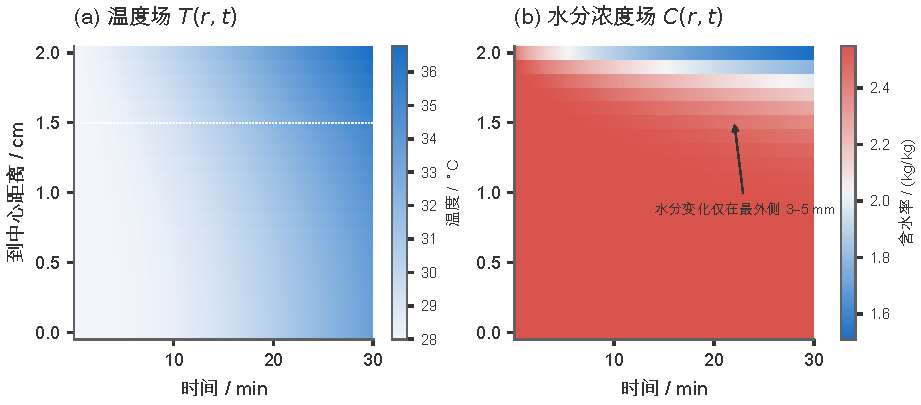
\includegraphics[width=\textwidth]{figs/d05_p1_fields.pdf}
  \caption{问题一的温度场 $T(r,t)$ 与水分浓度场 $C(r,t)$（$N=400$、
    $\Delta t=1$\,s）：30\,min 内热量已接近穿透整个截面，而水分变化
    仅发生在最外侧 $3\sim5$\,mm。}
  \label{fig:p1-fields}
\end{figure}

\begin{figure}[htbp]
  \centering
  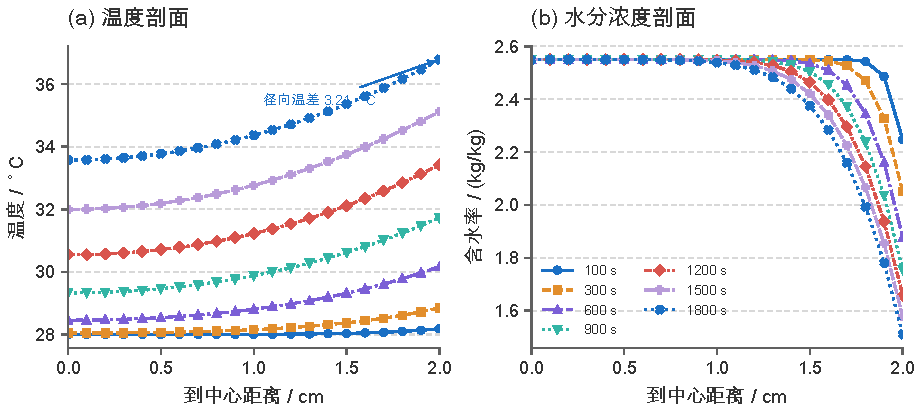
\includegraphics[width=\textwidth]{figs/d06_p1_profiles.pdf}
  \caption{问题一若干时刻的径向剖面族：(a) 温度剖面，$1800$\,s 时
    径向温差 $3.21\,^\circ$C；(b) 水分浓度剖面，梯度集中在表面附近。}
  \label{fig:p1-profiles}
\end{figure}

\subsection{本章小结}

本章建立了预热平衡阶段药材内部耦合传热传质的一维径向模型，
说明了问题一中热方程与水分方程解耦这一结构性质，给出无量纲特征数
$Bi=1.389$、$Bi_m=3.24$ 与特征扩散长度，
采用有限体积法配合后向 Euler 与 Picard 迭代完成求解，
守恒残差达机器精度，网格与时间步均已收敛。
计算结果表明：$1800$\,s 内药材温度整体上升并在径向上形成
$3.21\,^\circ$C 的温差，而水分脱除仅发生在表面约 $3\sim5$\,mm 的薄层内，
中心含水率没有可观测的变化。
完整结果保存在 \texttt{result1.xlsx} 中（时间 $1\sim1800$\,s、
径向 $0\sim2.0$\,cm 每 $0.1$\,cm，共 $1800\times21$ 个数据点，保留四位小数）。

\section{问题二：整个烘干过程的耦合传热传质模型}

\subsection{问题分析}

问题二要求建立\emph{整个}烘干过程（预热平衡 $+$ 恒温干燥，持续 $2\sim3$\,天）
药材温度与水分浓度的变化规律。与问题一的本质区别在于物性不再恒定：
附录 3 给出
\begin{equation}
  \rho=650+128C,\qquad
  c_p=1450+2736\frac{C}{C+1},\qquad
  k=0.21+0.38\frac{C}{C+1},
  \label{eq:p2-props}
\end{equation}
\begin{equation}
  D=2.4\times10^{-3}\,e^{-0.45/C}e^{-3850/T},
  \label{eq:p2-D}
\end{equation}
其中 $D$ 同时依赖含水率 $C$ 与温度 $T$（$T$ 取绝对温标 K），
$\rho$ 也随 $C$ 变化。因此水分方程中的扩散系数随温度演化，
而温度方程中的热容、导热系数随含水率演化，\textbf{两个方程必须联立求解}，
问题一中"热--质解耦"的结构性质不再成立。

\subsection{模型假设}

在问题一假设的基础上补充与修改：

\begin{enumerate}
  \item[(B1)] 预热平衡阶段与恒温干燥阶段使用同一组物性关系式
        \eqref{eq:p2-props}、\eqref{eq:p2-D}，两阶段的差别仅体现在
        烘房工况 $T_\infty$、$C_\infty$ 上；
  \item[(B2)] 恒温干燥阶段烘房工况恒定，取 $T_\infty=50\,^\circ$C、
        $C_\infty=0.05$\,kg/kg（依据见 §\ref{sec:bc}）；
  \item[(B3)] 问题二、三中不考虑药材尺寸变化（收缩由问题四处理），
        半径恒为 $R=2$\,cm；
  \item[(B4)] 对流换热系数与对流传质系数题面未给出，
        沿用附录 2 的 $h=25$\,W/(m$^2\cdot$K)、$h_m=8\times10^{-7}$\,m/s；
  \item[(B5)] 忽略汽化潜热，理由同问题一。
\end{enumerate}

\subsection{模型建立}

\subsubsection{控制方程}

圆柱坐标下的一维径向守恒方程：
\begin{equation}
  \rho(C)c_p(C)\frac{\partial T}{\partial t}
  =\frac{1}{r}\frac{\partial}{\partial r}
   \left(k(C)\,r\frac{\partial T}{\partial r}\right),
  \label{eq:p2-heat}
\end{equation}
\begin{equation}
  \frac{\partial C}{\partial t}
  =\frac{1}{r}\frac{\partial}{\partial r}
   \left(D\,r\frac{\partial C}{\partial r}\right).
  \label{eq:p2-mass}
\end{equation}

关于式 \eqref{eq:p2-mass} 的写法需要说明：未知量 $C$ 是干基含水率
（kg 水 / kg 干料），附录 3 给出的 $D$ 是针对该干基含水率拟合的有效
扩散系数（m$^2$/s），密度效应已被吸收进 $D$。需要说明的是，这里的
$\rho_d=\rho/(1+C)$ 随 $C$ 变化、在空间上并不均匀，并非“常数可约去”；
本文采用经典 Fick 口径，把该密度效应整体计入有效扩散系数 $D$，其代价
由第 \ref{sec:drymass} 节的干物质守恒检验量化（问题三 $+116\%$），
干基密度守恒口径的对照见表 \ref{tab:clos}（$-15.6\%$）。
体积密度 $\rho$ 仍以 $\rho c_p$ 的形式进入热方程。
具体误差分析见 §\ref{sec:closure}。

式 \eqref{eq:p2-heat} 采用\textbf{体积热容（apparent heat capacity）口径}：
时间导数作用在温度上，$\rho c_p$ 由当前时刻的 $C$ 取值，不把
$\rho c_p T$ 整体作为守恒量推进。问题一式 \eqref{eq:p1-heat}、问题四式
\eqref{eq:p4-heat} 与全部数值实现均采用同一形式，四个问题的能量口径一致。
在附录给出的 $\rho(C)$ 下，若写成 $\partial_t(\rho c_pT)$，会额外引入
$T\,\partial_t(\rho c_p)$ 项，其量级与主项相当（见附录 \ref{app:rho}），
本文不采用该口径。

\subsubsection{定解条件}

问题二的定解条件由初始条件与两端边界条件构成：

\begin{equation}
  T(r,0)=28\,^\circ\mathrm{C},\qquad C(r,0)=2.55\ \mathrm{kg/kg},
  \label{eq:p2-ic}
\end{equation}
\begin{equation}
  \left.\frac{\partial T}{\partial r}\right|_{r=0}=0,\qquad
  \left.\frac{\partial C}{\partial r}\right|_{r=0}=0,
  \label{eq:p2-center}
\end{equation}
\begin{equation}
  -k\left.\frac{\partial T}{\partial r}\right|_{r=R}
  =h\left(T_s-T_\infty(t)\right),
  \label{eq:p2-bcT}
\end{equation}
\begin{equation}
  -D\left.\frac{\partial C}{\partial r}\right|_{r=R}
  =h_m\left(C_s-C_\infty(t)\right).
  \label{eq:p2-bcC}
\end{equation}

\subsubsection{烘房工况的确定}
\label{sec:bc}

附件 1 只覆盖 $0\sim14400$\,s。对其末段 1\,h（$10800\sim14400$\,s）取平均，
得 $T_\infty=49.9989\,^\circ$C、$C_\infty=0.04999$\,kg/kg —— 与整数
$50\,^\circ$C、$0.05$\,kg/kg 几乎完全一致，说明这正是题目设定的恒温干燥工况。
因此边界条件取分段形式：
\begin{equation}
  T_\infty(t)=
  \begin{cases}
    \text{附件 1 线性插值}, & 0\le t\le 14400\ \mathrm{s},\\[2pt]
    50\,^\circ\mathrm{C}, & t>14400\ \mathrm{s},
  \end{cases}
  \label{eq:p2-Tinf}
\end{equation}
$C_\infty(t)$ 同理，$t>14400$\,s 后取 $0.05$\,kg/kg。

\subsection{模型求解}

\subsubsection{空间离散}

仍采用节点中心有限体积法，但此时每个控制体的"热容"随解变化
（$\rho c_p$ 依赖 $C$）。水分方程左端为 $\partial C/\partial t$；
界面上的扩散系数 $D$ 与导热系数 $k$ 由两侧节点值按算术平均构造，
与调和平均的对照见第 \ref{sec:face-avg} 节。

\subsubsection{时间离散与联立迭代}

时间方向用后向 Euler，非线性用 Picard 迭代：
\begin{equation}
  \begin{cases}
    \left(\bm{I}+\bm{A}_C^{(k)}\right)\bm{C}^{(k+1)}
      =\bm{b}\big(\bm{C}^{n},\bm{T}^{(k)}\big),\\[3pt]
    \left(\bm{I}+\bm{A}_T^{(k)}\right)\bm{T}^{(k+1)}
      =\bm{b}\big(\bm{T}^{n},\bm{C}^{(k+1)}\big),
  \end{cases}
  \qquad
  \big\|\cdot^{(k+1)}-\cdot^{(k)}\big\|_\infty<\varepsilon .
  \label{eq:p2-picard}
\end{equation}
取 $\varepsilon=10^{-11}$，通常 $2\sim3$ 次迭代收敛。每一步中两个方程各化为
一个三对角方程组，用追赶法在 $O(N)$ 时间内求解。

需要强调的一点：式 \eqref{eq:p2-picard} 右端的时间层 $n$ 必须是\textbf{本时间步
开始时}的状态，且在 Picard 迭代中保持不变；若误用上一迭代步的结果，
则每迭代一次就相当于再推进一个 $\Delta t$，数值解会比真实解快数倍。

\subsubsection{计算参数}

取 $N=200$（$r$ 方向）、$\Delta t=5$\,s，求解至中心含水率低于 $0.15$\,kg/kg。
收敛性检验见 §\ref{sec:p23-verify}。

\subsection{结果与分析}

表 \ref{tab:p2-T} 与表 \ref{tab:p2-C} 分别给出 3\,h 内每 $0.5$\,h 的温度与
水分浓度。

\begin{table}[htbp]
  \centering
  \caption{3 小时内药材的温度（单位：$^\circ$C）}
  \label{tab:p2-T}
  \begin{tabular}{cccccc}
    \toprule
    \multirow{2}{*}{时间/h} & \multicolumn{5}{c}{到药材中心的距离/cm} \\
    \cmidrule(lr){2-6}
     & 0     & 0.5   & 1.0   & 1.5   & 2.0 \\
    \midrule
    0.5 & 32.1966 & 32.3893 & 32.9727 & 33.9667 & 35.4176 \\
    1.0 & 40.3817 & 40.5536 & 41.0604 & 41.8785 & 42.9983 \\
    1.5 & 45.8436 & 45.9317 & 46.1901 & 46.6024 & 47.1376 \\
    2.0 & 48.4476 & 48.4855 & 48.5961 & 48.7715 & 49.0016 \\
    2.5 & 49.4653 & 49.4775 & 49.5121 & 49.5648 & 49.6614 \\
    3.0 & 49.8492 & 49.8550 & 49.8742 & 49.9098 & 49.9663 \\
    \bottomrule
  \end{tabular}
\end{table}

\begin{table}[htbp]
  \centering
  \caption{3 小时内药材的水分浓度（单位：kg/kg）}
  \label{tab:p2-C}
  \begin{tabular}{cccccc}
    \toprule
    \multirow{2}{*}{时间/h} & \multicolumn{5}{c}{到药材中心的距离/cm} \\
    \cmidrule(lr){2-6}
     & 0     & 0.5   & 1.0   & 1.5   & 2.0 \\
    \midrule
    0.5 & 2.5499 & 2.5488 & 2.5253 & 2.3257 & 1.6491 \\
    1.0 & 2.5255 & 2.4945 & 2.3577 & 2.0231 & 1.4713 \\
    1.5 & 2.3858 & 2.3254 & 2.1344 & 1.8021 & 1.3477 \\
    2.0 & 2.1708 & 2.1084 & 1.9237 & 1.6260 & 1.2312 \\
    2.5 & 1.9567 & 1.9007 & 1.7361 & 1.4721 & 1.1167 \\
    3.0 & 1.7663 & 1.7166 & 1.5703 & 1.3333 & 1.0082 \\
    \bottomrule
  \end{tabular}
\end{table}

\begin{figure}[htbp]
  \centering
  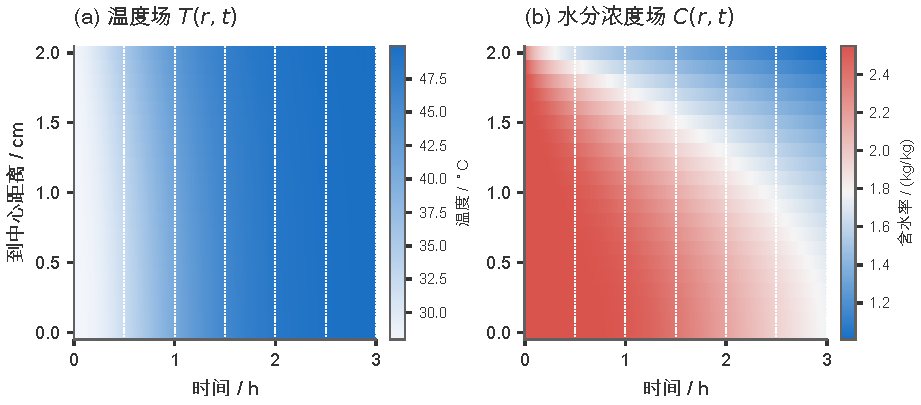
\includegraphics[width=\textwidth]{figs/d11_p2_fields.pdf}
  \caption{问题二的温度场 $T(r,t)$ 与水分浓度场 $C(r,t)$（$N=200$、
    $\Delta t=5$\,s）。温度在 $1$\,h 内已接近均匀（$3$\,h 时径向温差
    仅 $0.12\,^\circ$C），而水分浓度的高梯度区自表面向内推进：
    $3$\,h 时表面已降到 $1.0082$\,kg/kg，中心仍有 $1.7663$\,kg/kg，
    变化尚未波及 $r\lesssim1.0$\,cm 以内的芯部。}
  \label{fig:p2-fields}
\end{figure}

由结果可见三点。

第一，\textbf{升温呈“先慢后快”：前期略慢于问题一，随后迅速反超}。
问题一（附录 2）在 $1800$\,s 时中心为 $33.58\,^\circ$C，问题二为
$32.20\,^\circ$C，反而略低 $1.38\,^\circ$C。这与两问物性一致：附录 3 的
初始体积热容 $\rho c_p=3.33\times10^6$\,J/(m$^3\cdot$K) 大于附录 2 的
$2.13\times10^6$，初始热扩散率 $1.45\times10^{-7}$\,m$^2$/s 又小于
$1.69\times10^{-7}$\,m$^2$/s，故前期升温更慢。但水分快速脱除使
$\rho c_p$ 显著下降（$C$ 由 $2.55$ 降到 $0.15$ 时由 $3.33\times10^6$
降到 $1.21\times10^6$\,J/(m$^3\cdot$K)），热扩散率随之提高；同时式
\eqref{eq:p2-D} 中的 $e^{-3850/T}$ 使 $D$ 随升温急剧增大，两个效应互相
强化。到 $1.0$\,h 中心已达 $40.38\,^\circ$C，$3$\,h 达 $49.85\,^\circ$C，
后期升温明显快于问题一。

第二，\textbf{2.5\,h 后药材基本达到烘房温度}。$3$\,h 时中心 $49.85\,^\circ$C、
表面 $49.97\,^\circ$C，径向温差仅 $0.12\,^\circ$C。预热平衡阶段至此结束，
过程进入恒温干燥阶段。

第三，\textbf{水分脱除呈现出明显的"由表及里"次序}。$0.5$\,h 时中心基本未变
（$2.5499$），表面已降到 $1.6491$；$1$\,h 时中心才开始下降（$2.5255$）。
到 $3$\,h，表面降到 $1.0082$，而中心仍有 $1.7663$，径向梯度很大
（温度与水分浓度的时空场见图 \ref{fig:p2-fields}）。这说明过程始终由
内部扩散控制。

\subsection{模型检验}
\label{sec:p23-verify}

\subsubsection{求解器交叉验证}

把附录 3 的物性替换为附录 2 的常数物性后，本模型应当退化为问题一的模型。
实测：$t=1800$\,s 时温度场与独立的 \texttt{solve\_p1.py} 结果最大偏差为
$2.6\times10^{-12}\,^\circ$C，达到机器精度，说明离散格式实现正确。

\subsubsection{网格与时间步收敛性}

问题三的烘干时长同时受空间网格数 $N$ 与时间步长 $\Delta t$ 的影响。
本文不在此处罗列零散数据，而是把它们各自单列一节做系统对照：
径向网格数的影响见第 \ref{sec:grid} 节（表 \ref{tab:grid-N}），
时间步长的影响见第 \ref{sec:timestep} 节（表 \ref{tab:grid-dt}）。
两节同时给出本文（经典 Fick）口径与变密度口径的并排结果，
以便把"数值离散误差"与"模型口径差异"这两个来源分开。
简要结论：网格加密使烘干时长单调增加并近似一阶收敛；在本文采用的
算术平均格式内，$N=200$ 已进入网格无关区（与 $N=400$ 相差 $0.07\%$），
但\textbf{格式间的差别收敛更慢}——同为 $N=200$ 时调和平均仍偏高
$2.7\%$（第 \ref{sec:face-avg} 节），故“网格无关”应理解为格式内结论。
时间步的影响比网格小一个数量级，$\Delta t$ 由 $5$\,s 放宽到 $60$\,s
也仅改变 $0.10\%$。

\subsubsection{参数灵敏度分析}
\label{sec:sensitivity}

问题二至问题四的物性、换热与传质系数全部取自题面附录，其数值本身带有经验
公式的不确定度；而题面并未提供可用于标定这些参数的独立观测。因此，
"参数不准会不会改变结论"必须用灵敏度分析来回答。本文对三个关键系数
$h$、$h_m$、$D$ 分别作 $\pm20\%$ 扰动并重解问题三，结果见表
\ref{tab:sens}。

\begin{table}[htbp]
  \centering
  \caption{问题三烘干时长对关键参数的灵敏度（$N=100$，$\Delta t=5$\,s）}
  \label{tab:sens}
  \small
  \begin{tabular}{lccc}
    \toprule
    扰动方式 & 烘干时长/s & 烘干时长/h & 相对基准 \\
    \midrule
    基准值（$h=25$,\ $h_m=8\times10^{-7}$,\ $D$ 按附录 3） & 206365
      & 57.32 & --- \\
    $h$ 减小 $20\%$ & 206435 & 57.34 & $+0.03\%$ \\
    $h$ 增大 $20\%$ & 206320 & 57.31 & $-0.02\%$ \\
    $h_m$ 减小 $20\%$ & 212560 & 59.04 & $+3.0\%$ \\
    $h_m$ 增大 $20\%$ & 202555 & 56.27 & $-1.8\%$ \\
    $D$ 减小 $20\%$ & 252070 & 70.02 & $+22.2\%$ \\
    $D$ 增大 $20\%$ & 176175 & 48.94 & $-14.6\%$ \\
    \bottomrule
  \end{tabular}
\end{table}

表 \ref{tab:sens} 给出三个结论。

第一，\textbf{过程由内部水分扩散控制}。$D$ 是唯一强敏感参数：$D$ 变化
$20\%$，烘干时长在 $48.9\sim70.0$\,h 之间摆动，跨度接近一整天。

第二，\textbf{表面换热系数 $h$ 几乎不影响结果}（变化仅 $\pm0.03\%$）。
原因是热扩散率比水分扩散系数大 34 倍，温度场在整个过程中始终接近准稳态，
药材温度由空气温度直接决定，$h$ 的大小只是把这一平衡推进或推迟几分钟。

第三，\textbf{对流传质系数 $h_m$ 只带来 $2\sim3\%$ 的影响}，说明表面传质
阻力不是限制环节，内部扩散才是。

这组结果的实际意义是：\textbf{即使附录 2 给出的 $h$、$h_m$ 存在成倍误差，
问题三、问题四的结论也基本不变}，这正面回应了"参数无标定则模型不可信"的
质疑；同时也提示 $D$ 的取值口径与单位必须严格无误——附录 3、4 中 $D$ 的
经验公式以\textbf{绝对温标 $T$（K）}为自变量，若误用摄氏度将造成数量级错误。

\subsubsection{基于附件 2 实测数据的守恒性检验}
\label{sec:drymass}

前面的守恒检验、收敛性检验与交叉验证都属于模型内部的自治性检验。可用的
实测数据只有附件 1（烘房边界）与附件 2（药材半径），二者在模型中分别充当
激励与几何输入，并非独立的观测量。但其中仍有一个可检验的物理量：
\textbf{干物质质量守恒}。药材在烘干过程中只失去水分，固体骨架不流失，
故单位长度内的干料质量
\begin{equation}
  m_d(t)=\int_0^{R(t)}\frac{\rho\!\left(C\right)}{1+C}\,2\pi r\,\mathrm{d}r
  \label{eq:drysolid}
\end{equation}
应恒等于其初值。本文用已求得的 $C(r,t)$ 与附件 2 的实测 $R(t)$ 计算式
\eqref{eq:drysolid}，结果见表 \ref{tab:drymass}。

\begin{table}[htbp]
  \centering
  \caption{干物质质量的守恒性检验（相对初值）}
  \label{tab:drymass}
  \small
  \begin{tabular}{lcc}
    \toprule
    时刻 & 问题三（固定半径，附录 3） & 问题四（含收缩，附录 4） \\
    \midrule
    $12$\,h       & $+89\%$ & $-23.1\%$ \\
    $30$\,h       & $+110\%$ & $-13.8\%$ \\
    结束时刻       & $+116\%$ & $-10.9\%$ \\
    \bottomrule
  \end{tabular}
\end{table}

结果表明：两组给定数据在干物质守恒意义下存在固有张力。根源在于附录 3、4
的密度经验式本身已内含收缩效应——干基密度 $\rho/(1+C)$ 随含水率下降由
初值 $275$\,kg/m$^3$ 升至约 $600$\,kg/m$^3$（$C=0.15$ 的芯部点值为
$582$，体积加权平均约 $600$；$\rho_d\equiv\rho/(1+C)$ 的定义见
第 \ref{sec:rho} 节）；而问题二、三又要求
固定半径，二者叠加便隐含了干物质质量的增长。这是题面两组给定数据之间的
固有张力，并非本文模型引入，也不是"题目有错"——按第 \ref{sec:rho} 节
的分析，这两式各自都是合理的实验拟合式，只是隐含了不同的体积假设；
问题四因为直接采用了附件 2 的实际收缩，把偏差压缩到 $-11\%$ 以内
（12\,h 时一度到 $-23.1\%$，随后随半径停止收缩而回升）。

该结果说明两点。其一，本文给出的水分浓度场与烘干时长应理解为"题面给定
数据体系下的自洽解"，而非绝对预测值；其二，若要求严格的质量守恒，应改用
干基参考框架重写水分方程并放弃 $\rho(C)$ 的经验式，这已超出题面所给信息的
范围。本文如实报告该偏差，而不将其掩盖。

\subsubsection{水分方程口径的敏感性}

问题二起水分方程采用经典 Fick 形式
$\partial C/\partial t=\nabla\!\cdot\!(D\nabla C)$，其中 $C$ 为干基含水率、
$D$ 为针对该干基含水率拟合的有效扩散系数，体积密度 $\rho$ 只以
$\rho c_p$ 的形式进入热方程、不进入水分方程。题面未明确规定 $\rho$ 在水分
方程中的作用，为评估该口径对结论的影响，本文另按两种"把密度写回水分方程"的
常见口径重解问题三，结果见表 \ref{tab:clos}：其一为直接代入附录的体积密度
$\partial(\rho C)/\partial t=\nabla\!\cdot\!(\rho D\nabla C)$，
其等效扩散系数为 $\rho D/(\rho+C\rho')$；其二为按干基密度
$\rho_d=\rho/(1+C)$ 写守恒形式，其等效扩散系数为
$\rho_dD/(\rho_d+C\rho_d')$，在 $C_0$ 处约 $1.62D$、至判据
$C=0.15$ 处回落到 $1.11D$。

\begin{table}[htbp]
  \centering
  \caption{水分方程口径对问题三烘干时长的影响
    （$N=100$、$\Delta t=5$\,s；$N=200$ 时本文口径为 $57.42$\,h、
    变密度口径为 $61.02$\,h（$+6.3\%$）、干基密度守恒口径为 $48.47$\,h
    （$-15.6\%$）；三种口径的相对差在两套网格上完全一致）}
  \label{tab:clos}
  \small
  \begin{tabular}{lcc}
    \toprule
    水分方程口径 & 烘干时长/h & 相对基准 \\
    \midrule
    经典 Fick 形式 $\partial C/\partial t=\nabla\!\cdot\!(D\nabla C)$（本文）
      & 57.32 & --- \\
    $\partial(\rho C)/\partial t=\nabla\!\cdot\!(\rho D\nabla C)$
      & 60.93 & $+6.3\%$ \\
    干基密度守恒形式
      $\partial(\rho_dC)/\partial t=\nabla\!\cdot\!(\rho_dD\nabla C)$
      & 48.39 & $-15.6\%$ \\
    \bottomrule
  \end{tabular}
\end{table}

三种口径给出的烘干时长均在题面所述 $2\sim3$ 天区间内，四个问题的定性结论
不变；其中把体积密度 $\rho$ 写回水分方程会延长 $6.3\%$，改按干基密度
$\rho_d$ 的守恒形式则缩短 $15.6\%$。
后者与 $D$ 的 $\pm20\%$ 灵敏度同量级（$D$ 的扰动给出 $48.9\sim70.0$\,h），
但大于网格与时间步引入的数值误差（$\le1.6\%$ 与 $\le0.2\%$），
因此本文在此明确声明所采用的口径，以便复核。进一步的计算表明，
该口径差并不随数值参数漂移：在 $N=20\sim400$、$\Delta t=2\sim120$\,s
的全部组合中，把体积密度 $\rho$ 写回水分方程的口径相对本文稳定在 $+6.3\%$
（见第 \ref{sec:grid}、\ref{sec:timestep} 节）。

\section{烘干时间的确定（问题三）}

\subsection{问题分析}

烘干要求是"药材各处的\textbf{水分浓度应低于} $0.15$\,kg/kg"。
由于水分由表面向内部逐步脱除，整个过程中心处的含水率始终最高，
因此判据等价于
\begin{equation}
  t_{\mathrm{dry}}=\min\left\{t\ \middle|\
  \max_{0\le r\le R}C(r,t)<0.15\right\}
  =\min\left\{t\ \middle|\ C(0,t)<0.15\right\}.
  \label{eq:p3-criterion}
\end{equation}
数值上取求解过程中首次满足 $C(0,t)<0.15$ 的时刻。

\subsection{结果}

模型给出的烘干时长为
\begin{equation}
  t_{\mathrm{dry}}=206700\ \mathrm{s}=57.42\ \mathrm{h}=2.392\ \text{天}.
\end{equation}

该结果与题面"烘干过程一般持续 $2\sim3$ 天"的描述一致，
是对模型合理性的一个独立佐证。表 \ref{tab:p3} 给出每隔 $6$\,h 的
水分浓度分布。

\begin{table}[htbp]
  \centering
  \caption{药材烘干过程的水分浓度（单位：kg/kg）}
  \label{tab:p3}
  \begin{tabular}{cccccc}
    \toprule
    \multirow{2}{*}{时间/h} & \multicolumn{5}{c}{到药材中心的距离/cm} \\
    \cmidrule(lr){2-6}
     & 0     & 0.5   & 1.0   & 1.5   & 2.0 \\
    \midrule
    6  & 1.0171 & 0.9883 & 0.9016 & 0.7551 & 0.5329 \\
    12 & 0.4562 & 0.4432 & 0.4031 & 0.3298 & 0.1642 \\
    18 & 0.2989 & 0.2916 & 0.2687 & 0.2253 & 0.0846 \\
    24 & 0.2378 & 0.2327 & 0.2167 & 0.1855 & 0.0665 \\
    30 & 0.2058 & 0.2018 & 0.1891 & 0.1640 & 0.0599 \\
    36 & 0.1858 & 0.1825 & 0.1717 & 0.1503 & 0.0567 \\
    42 & 0.1720 & 0.1691 & 0.1596 & 0.1406 & 0.0549 \\
    48 & 0.1618 & 0.1591 & 0.1506 & 0.1333 & 0.0537 \\
    54 & 0.1538 & 0.1514 & 0.1436 & 0.1276 & 0.0530 \\
    烘干结束 & 0.1500 & 0.1477 & 0.1402 & 0.1248 & 0.0527 \\
    \bottomrule
  \end{tabular}
\end{table}

\subsection{结果分析}

从表 \ref{tab:p3} 可以看出烘干过程的三个典型阶段。

\textbf{快速干燥段（$0\sim12$\,h）}：含水率大幅下降，中心由 $2.55$ 降到
$0.4562$。这一段虽失水最快，却并非表面控制下的恒速干燥段：表面水分
始终充足、限制环节在内部扩散，故自始至终处于降速状态——中心含水率在
$0\sim6$\,h 下降 $1.53$，$6\sim12$\,h 只下降 $0.56$，速率已接近腰斩。

\textbf{降速干燥段（$12\sim36$\,h）}：速率明显放缓，中心由 $0.4562$ 降到
$0.1858$。表面含水率已接近空气平衡值（$0.05$ 附近），驱动力大幅衰减；
同时式 \eqref{eq:p2-D} 中 $e^{-0.45/C}$ 使 $D$ 随含水率降低而急剧减小，
内部水分越来越难迁移。

\textbf{极慢干燥段（$36\sim57.4$\,h）}：中心含水率由 $0.1858$ 缓缓逼近 $0.15$，
耗时约 $21$\,h，占全程的 $37\%$。这一段在工程上是最"不划算"的：
大量时间只换来很小的含水率下降。若对产品均匀性要求可以放宽，
适当延长或改用变温工艺会显著节能。

需要指出，判据由\textbf{中心}决定，而中心恰是最难干燥的位置。
$57.42$\,h 时有 $C(0)=0.1500$、$C(0.5\,\mathrm{cm})=0.1477$、
$C(2\,\mathrm{cm})=0.0527$，表面已干燥到接近平衡而中心刚刚达标，
内外含水率相差近三倍，干燥全过程的曲线见图 \ref{fig:p3}，
五个径向位置的历时曲线见图 \ref{fig:p3-family}。

\begin{figure}[htbp]
  \centering
  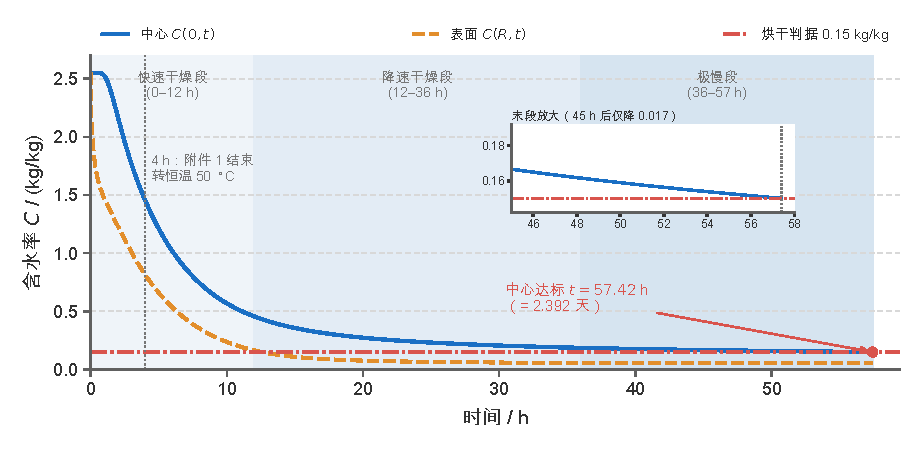
\includegraphics[width=\textwidth]{figs/d15_p3_curve.pdf}
  \caption{问题三干燥曲线：中心与表面水分浓度随时间的变化
    （$N=200$、$\Delta t=5$\,s，判据为各点 $C<0.15$\,kg/kg），
    右上角插图为 $45$\,h 之后的放大。}
  \label{fig:p3}
\end{figure}

\begin{figure}[htbp]
  \centering
  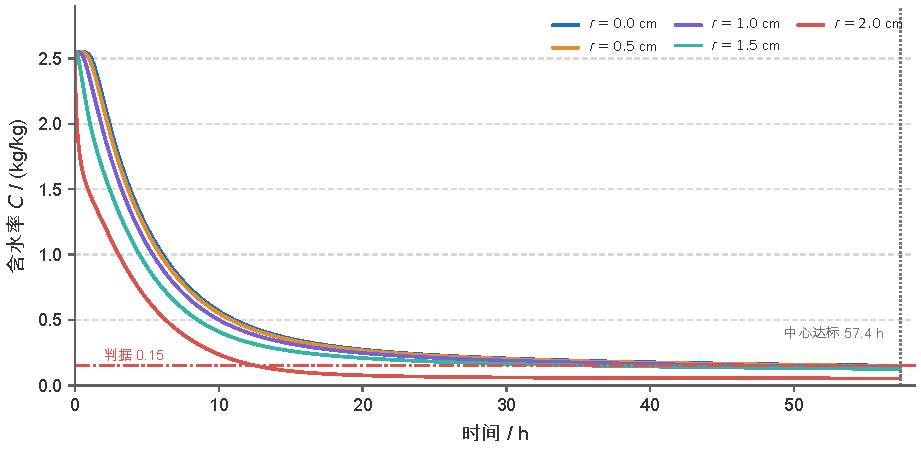
\includegraphics[width=\textwidth]{figs/d16_p3_family.pdf}
  \caption{问题三 5 个径向位置的含水率历时曲线（$N=200$、
    $\Delta t=5$\,s）：中心最后达标（$57.4$\,h），表面在 $12.6$\,h 即
    低于判据，此后由干壳控制。}
  \label{fig:p3-family}
\end{figure}

\section{考虑尺寸变化的烘干模型（问题四）}
\label{sec:p4}

\subsection{问题分析}

实际烘干中水分流失会引起药材收缩。附件 2 给出了半径随时间的实测变化：
$R$ 由 $2.000$\,cm 单调收缩至 $1.198$\,cm，收缩比 $0.599$，
对应截面积减为 $0.359$ 倍。

收缩带来了三个变化：其一，扩散路径变短，有利于干燥；
其二，表面几何面积减小，但对单位体积而言换热传质面积反而增大；
其三，计算区域随时间缩小，属于\textbf{动边界问题}，需要专门的坐标处理。

附件 2 的一个关键特征是收缩高度前置：
完成 $50\%$ 的收缩只需 $2.5$\,h，$90\%$ 只需 $10$\,h，$99\%$ 在 $22$\,h 内完成，
之后到 $72$\,h 半径几乎不再变化。也就是说，\textbf{收缩集中在干燥前期}，
而含水率的缓慢下降一直持续到 $50$\,h 之后。因此半径与含水率之间
不存在简单的线性关系，不宜用 $R=R_0 C/C_0$ 一类的经验式，
本文直接采用附件 2 的实测 $R(t)$。

\subsection{模型假设}

在问题二假设的基础上修改：

\begin{enumerate}
  \item[(C1)] 药材各点按比例均匀收缩，半径由附件 2 的 $R(t)$ 给定，
        即任意时刻的物理半径为 $r=\xi R(t)$，$\xi\in[0,1]$ 为贴体坐标；
  \item[(C2)] 物性改用附录 4 的经验公式
        \begin{equation}
          \rho=760+90C,\quad
          c_p=1850+2150\frac{C}{C+1},\quad
          k=0.12+0.20\frac{C}{C+1},
          \label{eq:p4-props}
        \end{equation}
        \begin{equation}
          D=4.2\times10^{-4}e^{-0.30/C}e^{-3850/T};
          \label{eq:p4-D}
        \end{equation}
  \item[(C3)] 初始半径 $R(0)=2.000$\,cm，与问题二一致，
        故初始条件仍为 $T=28\,^\circ$C、$C=2.55$\,kg/kg。
\end{enumerate}

\subsection{模型建立}

\subsubsection{贴体坐标变换：对流项精确抵消}

令
\begin{equation}
  \xi=\frac{r}{R(t)}\in[0,1],
\end{equation}
把移动区域 $[0,R(t)]$ 映射为固定区域 $[0,1]$。由于假设 (C1) 规定各点按
同一比例收缩，$\xi$ 同时是\textbf{材料坐标}：同一物质点在过程中保持
$\xi$ 不变，其物理速度为 $u=\xi\dot R$。

这里有一个容易被漏掉、但决定方程形式的关键点。在物理坐标下，温度与水分
满足带骨架对流的守恒关系，时间导数应写成物质导数
\begin{equation}
  \frac{\mathrm{D}}{\mathrm{D}t}
  =\left.\frac{\partial}{\partial t}\right|_{r}
   +u\,\frac{\partial}{\partial r},
  \label{eq:p4-material-deriv}
\end{equation}
而坐标变换本身给出
\begin{equation}
  \left.\frac{\partial}{\partial t}\right|_{r}
  =\left.\frac{\partial}{\partial t}\right|_{\xi}
   -\frac{\xi\dot R}{R}\frac{\partial}{\partial\xi},
  \qquad
  \frac{\partial}{\partial r}=\frac{1}{R}\frac{\partial}{\partial\xi},
  \label{eq:p4-transform}
\end{equation}
其中 $\dot R=\mathrm{d}R/\mathrm{d}t<0$。两式相加，右端第二项与
$u\,\partial_r=\dfrac{\xi\dot R}{R}\partial_\xi$ \textbf{恰好抵消}：
\begin{equation}
  \frac{\mathrm{D}}{\mathrm{D}t}
  =\left.\frac{\partial}{\partial t}\right|_{\xi}.
  \label{eq:p4-cancel}
\end{equation}
也就是说，材料坐标下的时间导数本身就是物质导数，方程中\emph{不应}再出现
任何额外的“挤压”对流项；算子的空间部分只须把 $r=\xi R$ 代入散度。代入
式 \eqref{eq:p2-heat}、\eqref{eq:p2-mass} 并整理，得
\begin{equation}
  \rho c_p\,\xi R^2\frac{\partial T}{\partial t}
  =\frac{\partial}{\partial\xi}
   \left(k\,\xi\frac{\partial T}{\partial\xi}\right),
  \label{eq:p4-heat}
\end{equation}
\begin{equation}
  \xi R^2\frac{\partial C}{\partial t}
  =\frac{\partial}{\partial\xi}
   \left(D\,\xi\frac{\partial C}{\partial\xi}\right).
  \label{eq:p4-mass}
\end{equation}
与问题二、三的方程组相比，唯一的差别是度量因子由 $R_0^2$ 变成
$R(t)^2$、表面边界条件多一个 $R$。水分方程仍不含体积密度 $\rho$，
但在问题四里这一步是\textbf{严格推出}的而非沿用：由假设 (C1) 各点按同一
比例收缩，任意物质微元的体积以同一因子缩放，干物质质量守恒使
$\rho_d=\rho/(1+C)$ 只随时间变化、在空间上\textbf{均匀}。于是材料坐标下
$\rho_d\,\partial_tC|_\xi=\frac1r\partial_r\!\left(r\rho_dD\,\partial_rC
\right)=\rho_d\,\frac1r\partial_r\!\left(rD\,\partial_rC\right)$，
$\rho_d(t)$ 可从散度中提出并在两侧约去，得到式 \eqref{eq:p4-mass}；
这与 $\rho_d$ 是否随时间变化无关。这样四个问题共用同一个物质输运口径，
问题四与问题三的差异\emph{只有几何}一个因素，二者的比较才是严格单因素的。
若令 $\dot R\equiv0$，式 \eqref{eq:p4-heat}、\eqref{eq:p4-mass} 严格退化
为问题二的方程组。

\subsubsection{定解条件}

初始条件与中心对称条件同式 \eqref{eq:p2-ic}、\eqref{eq:p2-center}。
表面 $\xi=1$ 处边界条件形式不变：
\begin{equation}
  -k\left.\frac{\partial T}{\partial\xi}\right|_{\xi=1}
  =hR\left(T_s-T_\infty\right),\qquad
  -D\left.\frac{\partial C}{\partial\xi}\right|_{\xi=1}
  =h_mR\left(C_s-C_\infty\right).
  \label{eq:p4-bc}
\end{equation}

\subsubsection{$R(t)$ 的处理}

附件 2 为每 $1800$\,s 一个点的离散数据。$R(t)$ 直接进入度量因子
$1/R^2$ 与表面边界条件，且第 \ref{sec:p11-crosscheck} 节要用它的导数
$\dot R$ 反演收缩速率。若直接线性插值，$R$ 的斜率在节点处跳变，会让
进入方程系数的几何量出现阶梯；若用差分估计 $\dot R$，噪声会被放大
$1/\Delta t$ 倍。因此本文采用\textbf{单调三次 Hermite 插值
（PCHIP，Fritsch--Carlson 构造）}\cite{ref-fc}，它既保证 $C^1$ 连续，又保持数据的
单调性、不产生过冲。
收缩终止的时刻由数据本身决定，无需外推。

\subsection{数值实现}

空间离散仍用节点中心有限体积，但控制体权重变为
$w_i=\int\xi\,\mathrm{d}\xi$，即
\begin{equation}
  w_0=\frac{h^2}{8},\qquad w_i=\xi_i h\ (1\le i\le N-1),\qquad
  w_N=\frac{h(1-h/4)}{2}.
\end{equation}
收缩只通过每个时间步的 $R(t_n)$ 进入度量因子与表面边界条件，
离散格式与问题二逐项相同；时间方向与非线性处理同问题二，
取 $N=200$、$\Delta t=5$\,s。

\subsection{结果}

模型给出的烘干时长为
\begin{equation}
  t_{\mathrm{dry}}=183885\ \mathrm{s}=51.08\ \mathrm{h}=2.128\ \text{天},
\end{equation}
比问题三的 $57.42$\,h 缩短了约 $11.0\%$。但该差值同时包含物性由附录 3
换为附录 4 的影响，\textbf{不能全部归因于收缩}；收缩的独立贡献须在同一
物性下比较，见下节。

\begin{table}[htbp]
  \centering
  \caption{药材烘干过程的水分浓度（含收缩，单位：kg/kg）}
  \label{tab:p4}
  \small
  \begin{tabular}{ccccccc}
    \toprule
    \multirow{2}{*}{时间/h} & \multicolumn{5}{c}{到药材中心的距离/cm}
      & \multirow{2}{*}{药材表面} \\
    \cmidrule(lr){2-6}
     & 0     & 0.5   & 1.0   & 1.5   & 2.0 & \\
    \midrule
    6  & 1.7188 & 1.5371 & 1.0222 & —— & —— & 0.4205 \\
    12 & 0.7375 & 0.6544 & 0.4082 & —— & —— & 0.1669 \\
    18 & 0.4087 & 0.3686 & 0.2397 & —— & —— & 0.0892 \\
    24 & 0.2851 & 0.2610 & 0.1789 & —— & —— & 0.0673 \\
    30 & 0.2263 & 0.2094 & 0.1492 & —— & —— & 0.0595 \\
    36 & 0.1928 & 0.1796 & 0.1316 & —— & —— & 0.0560 \\
    42 & 0.1712 & 0.1603 & 0.1199 & —— & —— & 0.0541 \\
    48 & 0.1561 & 0.1468 & 0.1115 & —— & —— & 0.0530 \\
    烘干结束 & 0.1500 & 0.1413 & 0.1080 & —— & —— & 0.0526 \\
    \bottomrule
  \end{tabular}
\end{table}

表 \ref{tab:p4} 中 $1.5$\,cm 与 $2.0$\,cm 两列以"——"表示，
原因是半径收缩至 $1.5$\,cm 以下之后（约 $3.6$\,h）这些位置已不在药材内部，
水分浓度无定义（移动边界下的含水率场见图 \ref{fig:p4-field}）。
这也是题面表 6 用"药材表面"而非固定距离作为末列的原因：表面位置本身
是随时间移动的。

\begin{figure}[htbp]
  \centering
  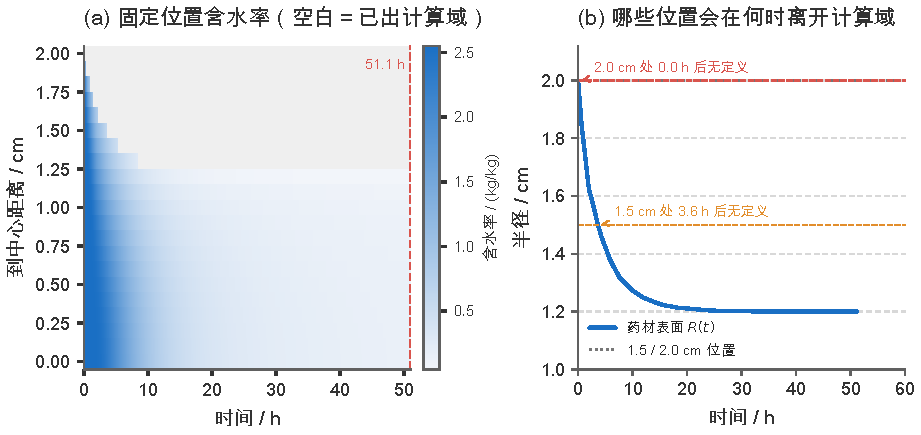
\includegraphics[width=\textwidth]{figs/d20_p4_field.pdf}
  \caption{问题四移动边界下的含水率场：(a) 固定位置含水率，
    空白表示该位置已随收缩离开计算域；(b) 各半径位置的失效时刻，
    表面由 $2.0$\,cm 收缩到 $1.198$\,cm。}
  \label{fig:p4-field}
\end{figure}

\subsection{收缩对烘干时长的影响}

为分离收缩的贡献，用附录 4 的同一组物性、\textbf{同一套水分方程口径}，
只把半径固定为 $R\equiv2$\,cm 再求解一次，得烘干时长
$467260$\,s $=5.41$ 天；计入收缩后为 $2.13$ 天，缩短为原来的 $39.4\%$。
因为两次求解只差几何一个因素，这个差值可以全部归因于收缩。

这一效应可从两个层面理解：扩散路程由 $R$ 缩短至 $0.6R$，
特征扩散时间按 $R^2$ 计减少到 $36\%$；
单位体积的表面积按 $1/R$ 计增大约 $1.67$ 倍，
表面交换能力相对增强。

这一结论有明确的工程含义：\textbf{忽视收缩会严重高估烘干时长}
（本例中忽略收缩的预测时长为计入收缩时的 $2.54$ 倍，即高估约 $154\%$）。
若按不考虑收缩的结果安排生产，
会造成过度干燥、能耗浪费，甚至因干裂而降低药材品质。
收缩历程与两种情形的对照见图 \ref{fig:p4}。

\begin{figure}[htbp]
  \centering
  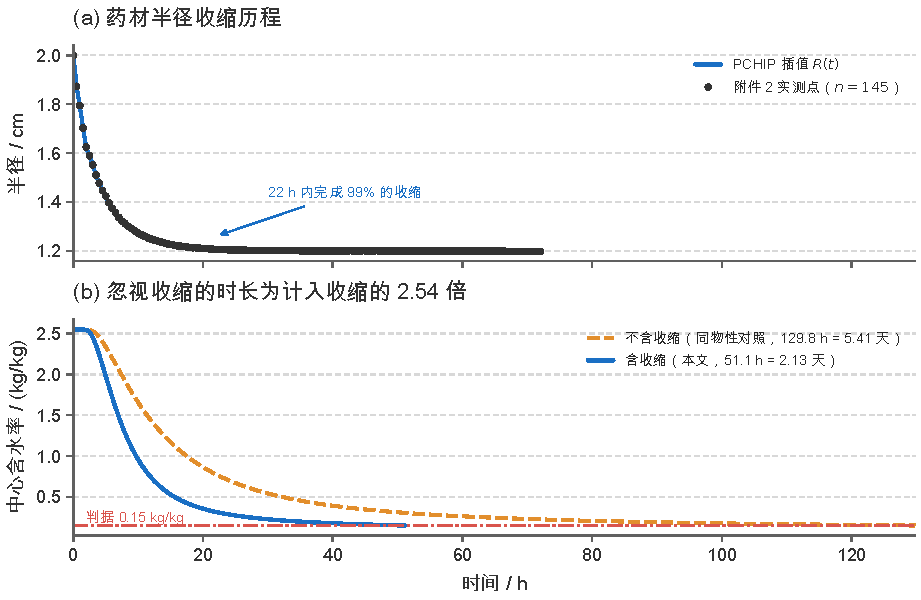
\includegraphics[width=0.90\textwidth]{figs/d19_p4_shrink.pdf}
  \caption{问题四：收缩历程与烘干时长的对照
    （附录 4 物性，$N=200$、$\Delta t=5$\,s）。
    (a) 附件 2 的实测半径（$n=145$，间隔 1800\,s，实测点以散点示出）
    与保单调三次 Hermite 插值曲线；插值后 $\dot R\le0$ 恒成立、
    无过冲。(b) 中心水分浓度随时间的变化：含收缩时 51.08\,h 达标，
    固定半径的对照工况需 129.79\,h，收缩使烘干时长缩短约 61\%。
    两图均为确定性数值结果，不含统计误差。}
  \label{fig:p4}
\end{figure}

\subsection{模型检验}

模型检验从退化一致性、单调性与守恒性三方面进行：

\begin{enumerate}
  \item \textbf{退化检验}：令 $\dot R\equiv0$ 并把附录 4 物性替换为
        附录 2 的常数物性，式 \eqref{eq:p4-heat}、\eqref{eq:p4-mass}
        退化为问题一模型，程序实测退化解与问题一解完全一致，
        说明材料坐标下的动区域离散实现正确。

  \item \textbf{口径一致性检验}：问题四的水分方程为式
        \eqref{eq:p4-mass}，与问题二、三的经典 Fick 口径完全相同，
        只有度量因子与表面边界条件带 $R(t)$；因此问题四与问题三的
        对照是严格的单因素（几何）对照。
  \item \textbf{单调性检验}：PCHIP 插值后的 $R(t)$ 单调递减，
        未出现插值过冲引起的非物理膨胀。
  \item \textbf{合理性检验}：收缩使烘干时长缩短，
        与"扩散路径变短有利于干燥"的物理预期一致；
        问题三 $57.42$\,h、问题四 $51.08$\,h 均落在题面所述
        $2\sim3$ 天区间内。
\end{enumerate}

\section{模型的检验与灵敏度分析}
\label{sec:verify-num}

本文对数值方案做了三类系统检验：空间网格 $N=20\to400$、时间步
$\Delta t=2\sim120$\,s、界面扩散系数取法（算术／对数／调和平均）。
完整对照数据、逐档收敛过程与讨论见附录 \ref{app:num-detail}，
这里只列对结论有影响的四条。

\begin{enumerate}
  \item \textbf{报告网格不等于求解网格。}题面 $0.1$\,cm 的输出网格对应
        $N=20$，直接用它求解会把烘干时长低估 $1.6\%$（$203335$\,s 对
        $206700$\,s）；本文在 $N=200$ 上求解后再插值到输出网格。
  \item \textbf{本文配置下网格已足够密。}$N=200$ 与 $N=400$ 的烘干时长
        相差 $0.07\%$，相邻增量逐次减半；时间步在 $60$ 倍跨度内的最大
        影响不超过 $0.2\%$。
  \item \textbf{格式无关性慢于格式内收敛。}界面取法在 $N=200$ 上仍有
        $2.7\%$ 的残差（调和平均相对算术平均，$58.96$\,h 对
        $57.42$\,h），加密到 $N=400$ 后降到 $0.4\%$。因此"网格无关"只是
        算术平均格式内的结论，界面取法的不确定性在误差排序中高于网格。
  \item \textbf{口径差与数值参数无关。}把体积密度写回水分方程使烘干时长
        稳定延长 $+6.3\%$，在 $N=20\sim400$、$\Delta t=2\sim120$\,s 的
        20 组参数组合下不漂移，说明它属模型口径而非离散误差。
\end{enumerate}

\section{收缩的建模判据与代价}
\label{sec:shrink-criterion}

\subsection{本节要回答的问题}

四个问题用了两套密度经验式：问题二、三用附录 3 的 $\rho=650+128C$，
问题四用附录 4 的 $\rho=760+90C$；对收缩的处理也不同——前三问取固定半径，
问题四计入附件 2 的实测收缩。这一分工在题面中已经给定，但有一个问题值得
正面回答：\textbf{能否只看经验式的系数，就判断某一问该不该考虑收缩？}
本节说明答案是肯定的，判据只依赖一个无量纲量——\textbf{斜率与截距之比}
$r\equiv b/a$；并把"考虑收缩"的代价量化成烘干时长的改变量，从而给出
一条可以照搬到假设一节的分层规则。

\subsection{收缩几何只由斜率截距比决定}

以 $1$\,kg 干物质为基准，由恒等式 $\rho=\rho_d(1+C)$ 与 $\rho_d=m_d/V$
立得单位干物质体积
\begin{equation}
  V(C)=\frac{1+C}{\rho(C)}=\frac{1+C}{a+bC},
  \label{eq:p11-v}
\end{equation}
于是从初态 $C_0$ 到当前 $C$ 的体积比为
\begin{equation}
  \frac{V(C)}{V(C_0)}
  =\frac{(1+C)(a+bC_0)}{(1+C_0)(a+bC)}
  =\frac{(1+C)(1+rC_0)}{(1+C_0)(1+rC)},
  \qquad r=\frac{b}{a},
  \label{eq:p11-ratio}
\end{equation}
分子分母同除以 $a$ 后\textbf{截距被完全约去}。

\textbf{命题（单参数约化）}\quad 相对体积 $V(C)/V(C_0)$、由它决定的相对线尺度
以及动边界 $R(t)$ 的形状，都只通过 $r=b/a$ 依赖密度经验式；截距 $a$ 与系数的
绝对大小不进入几何。这说明把经验式整体等比例放大或缩小（$a$、$b$ 同乘一个
常数）不改变任何收缩量。几何约定上，本文问题四取\textbf{长度不变、只缩半径}，
故 $R/R_0=[V/V_0]^{1/2}$；若按各向同性收缩则为立方根，两者相差约三分之一
（附录 3 的绝干线收缩由 $35.0\%$ 变为 $24.9\%$）。全文只用前一种口径。

两套经验式的 $r$ 分别为 $r_3=128/650=0.197$ 与 $r_4=90/760=0.118$。
它与附件 2 实测收缩的对照可由端点值给出。定义端点收缩系数
\begin{equation}
  \beta\equiv\frac{\Delta V/V_0}{\varepsilon_w^0}
  =\frac{1-V(0)/V(C_0)}{\varepsilon_w^0},\qquad
  \varepsilon_w^0=\frac{C_0}{\rho_w^0}\cdot\frac{a+bC_0}{1+C_0},
  \label{eq:p11-beta}
\end{equation}
即“绝干时总体积收缩量与初始水体积之比”。由式 \eqref{eq:p11-ratio} 可解出
$\beta(r)=(\rho_w^0/a)(1-r)/(1+rC_0)$，代入得 $\beta_3=0.822$、
$\beta_4=0.891$。$\beta$ 携带绝对物理含义、需要密度尺度 $a$ 与水的真密度；
而"该不该忽略收缩"是纯几何决策，只有 $r$ 是必要的。

\subsection{两级判据}
\label{sec:p11-criteria}

相对体积 $V(C)/V(C_0)$ 只通过 $r=b/a$ 依赖密度经验式，由此可把
“该不该考虑收缩”写成求解之前即可计算的判据。完整闭式推导、阈值表与
参数扫描见附录 \ref{app:shrink}，结论有两条。

\textbf{（1）几何判据。}给定半径容差 $\varepsilon$ 与工作窗口
$[C_{\min},C_0]$，忽略收缩安全当且仅当 $r\ge r^\ast(\varepsilon,C_{\min})$。
$5\%$ 径向容差下，预热窗口（$C:2.55\to2.0$）的阈值为 $0.164$：附录 3
（$r_3=0.197$）通过，该窗口内线收缩仅 $4.57\%$；\textbf{附录 4
（$r_4=0.118$）已经越界}，同一窗口的线收缩为 $5.68\%$，略超容差。
问题二窗口（$C:2.55\to1.364$）阈值升到 $0.507$、全程窗口（$C\to0.15$）
升到 $0.838$，两式均已落到阈值之下——\textbf{无论用哪套物性，深干燥段的
收缩都不可忽略}。这正是本文把问题四单列的原因，也说明"预热段可以忽略
收缩"只在附录 3 的物性下严格成立。

\textbf{（2）时长判据。}把半径容差升级为烘干时长误差 $\Delta$，
$\Delta\le5\%/10\%/20\%$ 分别要求 $r\ge0.913/0.835/0.704$，比几何判据更严
（半径以平方进入特征扩散时间）。题面两式按任一口径都远低于阈值；
附录 \ref{app:shrink} 的参数扫描还给出：固定几何时 $r$ 对烘干时长几乎无
影响（全变程 $0.24\%$），一旦计入收缩，影响被放大到 $+3\%\sim+169\%$。

\subsection{三个开关对烘干时长的相对重要性}

把上面的分析落到本问的物性体系上，可以给出三个"开关"对烘干时长的实际影响
（表 \ref{tab:p11-geom}）。所有数字都保持物性体系不变，只切换被测的那个量。

\begin{table}[htbp]
  \centering
  \caption{建模开关对烘干时长的影响（物性体系固定，只切换被测项）
    。"口径"一列见第 \ref{sec:closure} 节，"几何"三行用附录 3 物性、
    $N=100$、$\Delta t=5$\,s 求解}
  \label{tab:p11-geom}
  \small
  \begin{tabular}{llcc}
    \toprule
    开关 & 取值 & 烘干时长 & 相对基准 \\
    \midrule
    几何 & 固定半径 $R_0$（本文问题二/三） & $57.32$\,h & --- \\
         & 由 $\rho=a+bC$ 反演 $R(C)$ 自洽闭合 & $29.45$\,h & $-48.6\%$ \\
         & 附件 2 实测 $R(t)$（问题四的几何） & $23.85$\,h & $-58.4\%$ \\
    \midrule
    水分方程口径 & 经典 Fick（本文） & $57.32$\,h & --- \\
                 & 体积密度守恒 $\partial(\rho C)/\partial t$ & $60.93$\,h
      & $+6.3\%$ \\
    \midrule
    参数 & $D\pm20\%$（第 \ref{sec:sensitivity} 节） & $48.9\sim70.0$\,h
      & $-15\%\sim+22\%$ \\
    \bottomrule
  \end{tabular}
\end{table}

三点结论。

\textbf{（1）"是否考虑收缩"是三者中影响最大的开关。}在同一套物性下，
计入由经验式反演的收缩使烘干时长缩短 $48.6\%$，计入实测收缩缩短 $58.4\%$；
而把体积密度写回水分方程只延长 $6.3\%$、改按干基密度守恒反而缩短
$15.6\%$，$D$ 变化 $\pm20\%$ 带来 $-15\%\sim+22\%$。\textbf{收缩效应比
口径效应（$6.3\%\sim15.6\%$）大 $3$ 倍以上}，也大于参数不确定度。

\textbf{（2）"是否考虑 $\rho$"与"是否考虑收缩"不是两个独立的开关。}
由恒等式 $\rho=\rho_d(1+C)$、$\rho_d=m_d/V$ 可知：几何固定时把体积密度写进
水量守恒，等价于要求 $V$ 不变而 $\rho$ 随 $C$ 变，这会使干物质质量随干燥
过程增长——第 \ref{sec:drymass} 节的检验给出问题三 $+116\%$ 的漂移。
所以严格地说，\textbf{只有"几何收缩 + $\rho$ 守恒形式"这一组合是自洽的}；
固定几何下的正确做法是让 $\rho_d$ 在方程两侧约去（本文问题二、三），
而不是把 $\rho$ 硬写进水分方程。

\textbf{（3）两条收缩路径给出同一量级、不同数值。}由经验式反演的收缩
（$29.45$\,h）与附件 2 实测收缩（$23.85$\,h）相差 $23\%$——
两者总量接近，但收缩的时间路径不同。这解释了为什么问题四必须以实测
$R(t)$ 为准（见下节），也界定了判据的适用边界：$r$ 给出的是收缩的
\textbf{总量律}，而不是\textbf{时间律}。

\subsection{与附件 2 实测收缩的对照}
\label{sec:p11-crosscheck}

上述判据以经验式隐含的收缩为基础，把它与附件 2 的实测半径对照，
可以检验这条判据是否可信。图 \ref{fig:geo-shrink} 把两者画在同一坐标系中，
结果分两层。

\textbf{总量上互证。}在\textbf{径向等长}口径下，把附录 4（$r=0.118$）的
密度经验式外推到绝干，得半径 $1.211$\,cm，与附件 2 的实测终半径
$1.198$\,cm 只差 $1.1\%$；换成体积收缩比是 $63.3\%$ 对 $64.1\%$
（相对差 $1.2\%$）。附录 3 的 $1.301$\,cm 则偏 $+8.6\%$。需要说明的是，
$1.1\%$ 是“外推到绝干”与“实测已进入平台”的比较；若改按\textbf{同一
含水率}比较——取问题四结束时刻的体积加权平均含水率 $\bar C=0.117$——
经验式给出 $1.271$\,cm，与实测 $1.200$\,cm 相差 $5.6\%$
（图 \ref{fig:geo-shrink}b）。两个数字含义不同：前者说明两组数据隐含的
\emph{收缩总量}一致，后者说明二者的\emph{收缩路径}不同。据此可以说，
题面为问题四同时给出的两组数据（附件 2 的 $R(t)$ 与附录 4 的 $\rho(C)$）
在“干燥全程能缩到多小”这一点上互相印证，问题四把二者搭配使用是有依据的。

\textbf{路径上互补。}把问题四求得的场按体积加权平均含水率折算成比体积，
与由 $\rho(C)$ 反推的比体积在\textbf{同一含水率}下比较，可见附件 2 的实测
收缩在时间上高度前置：$50\%$ 的收缩在 $2.5$\,h 内完成、$99\%$ 在 $22$\,h
内完成，此后半径几乎不变；而 $\rho$ 律要求收缩与含水率同步下降。
两者在同一含水率下的比体积相差 $10.6\%\sim22.4\%$（图 \ref{fig:geo-shrink}）。
这不是矛盾：$\rho(C)$ 是平衡态的比体积关系，附件 2 记录的是实际干燥历程，
二者的差别恰是"收缩不是平均含水率的单值函数"的体现。也正是这个差别，
使得问题四必须采用实测 $R(t)$ 而不是自行反演一条收缩律。

\begin{figure}[htbp]
  \centering
  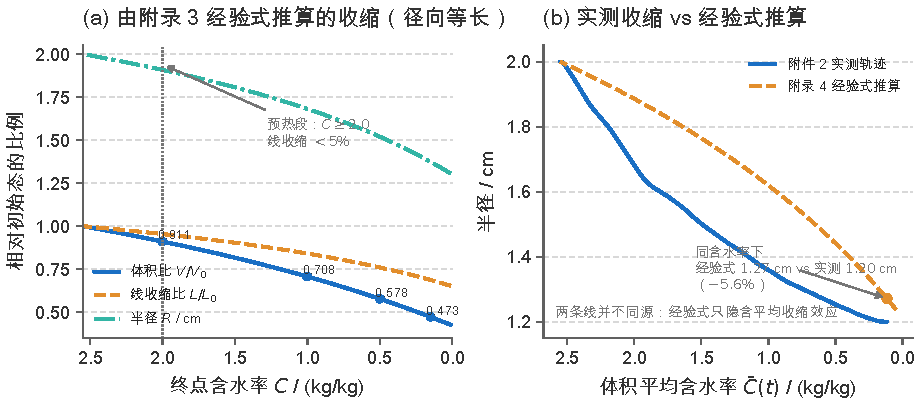
\includegraphics[width=\textwidth]{figs/d29_geo_shrink.pdf}
  \caption{(a) 由附录 3 经验式推算的几何收缩：体积比 $V/V_0$、
    线收缩比 $L/L_0$ 与对应半径随终点含水率的变化；$C\ge2.0$ 时线收缩不足
    $5\%$（径向等长口径）。(b) 由 $\rho(C)$ 反推的 $R(C)$ 与附件 2 实测
    $R$–$C$ 轨迹的对照（横轴为体积加权平均含水率 $\bar C$）：同一含水率下
    经验式比实测偏大约 $5.6\%$，外推到绝干则只差 $1.1\%$；路径上前者与
    含水率同步、后者高度前置。}
  \label{fig:geo-shrink}
\end{figure}

\subsection{回看四个问题：分层规则}

综合两级判据与代价量化，本文对收缩的处理可以写成一条分层规则，
每一层都有定量依据：

\begin{enumerate}
  \item \textbf{问题一（预热段，$C$ 由 $2.55$ 降到约 $2.0$）}：该问按题面给定的
        常物性与固定几何求解，附录 2 只给出一个常数密度，并未给出可用于本判据的
        $\rho=a+bC$ 经验式，因此不把 $r=b/a$ 判据外推到该问。对附录 3、4 而言，
        同一窗口在 5\% 径向容差下分别为“通过（$4.57\%$）”与“轻微越界
        （$5.68\%$）”，可见“预热段收缩可忽略”应理解为\textbf{题面分工下的
        近似}，而不是由两套变物性经验式共同严格保证的结论。
  \item \textbf{问题二（3\,h 窗口，$C$ 平均降到 $1.364$）}：该窗口在 5\% 容差
        下阈值 $r^\ast=0.507$，而两套物性的 $r$ 分别为 $0.197$ 与 $0.118$，
        已在阈值之下，说明这一窗口内收缩\textbf{不再是可以随手忽略的小量}。
        本文按题面分工仍取固定半径（假设 B3），但把它显式声明为一条简化，
        并以第 \ref{sec:sensitivity} 节的灵敏度与本节表 \ref{tab:p11-sweep}
        量化其代价。
  \item \textbf{问题三（全程，$C\to0.15$）}：全程窗口的 5\% 阈值升到
        $r^\ast=0.838$，两套物性都远在阈值之下；时长口径下 $\Delta$ 达 $95\%$。
        这是三者中唯一"必须考虑"的量级，也正是题目把尺寸变化单列为问题四的
        原因。
  \item \textbf{问题四（全程，几何由题面给出）}：题面在这一问同时提供了
        附件 2 的实测 $R(t)$ 与附录 4 的 $\rho(C)$，且明确要求计入尺寸变化。
        按本节判据，$r_4=0.118$ 远低于阈值，故必须建模；而实测收缩比经验式
        隐含的收缩更强，因此本文采用实测 $R(t)$ 并引入贴体坐标。
\end{enumerate}

这样一来，"问题一至三取固定几何、问题四计入收缩"就不再是两套互不相干的
假设，而是同一条判据在四个不同窗口上的取值结果。同时也要如实指出：
\textbf{按判据，问题二、三的窗口已经越界}，本文在这些问题上取固定半径是
题面分工下的选择，其代价已在表 \ref{tab:p11-geom} 中给出，
而不是"因为误差很小所以可以忽略"。

\subsection{小结}

本节的可迁移结论是：收缩几何只由 $r=b/a$ 决定，据此可在求解之前先验判断
某问能否忽略收缩（几何判据），并可进一步给出时长口径的阈值；在本问的物性
体系下，收缩对烘干时长的影响（$-49\%\sim-58\%$）比水分方程口径
（$6.3\%\sim15.6\%$）大 $3$ 倍以上，也大于 $D$ 的 $\pm20\%$ 不确定度。
由 $r$ 反推的绝干半径与附件 2 实测终半径相差 $1.1\%$，说明判据与实测收缩
在总量上互证、在路径上互补（相差 $10.6\%\sim22.4\%$），这正是问题四取
实测 $R(t)$ 的理由。

\section{结果汇总与交付说明}

四个结果文件均按附件 3 模板的格式保存，所有数值保留四位小数，其规模与
内容见表 \ref{tab:files}：

\begin{table}[htbp]
  \centering
  \caption{结果文件一览}
  \label{tab:files}
  \small
  \begin{tabular}{llll}
    \toprule
    文件 & 工作表 & 时间范围与间隔 & 规模 \\
    \midrule
    \texttt{result1.xlsx} & 温度、水分浓度 & $1\sim1800$\,s，每 $1$\,s & $1800\times21$ \\
    \texttt{result2.xlsx} & 温度、水分浓度 & $1\sim206700$\,s，每 $1$\,s & $206700\times21$ \\
    \texttt{result3.xlsx} & 水分浓度 & $60\sim206700$\,s，每 $60$\,s & $3445\times21$ \\
    \texttt{result4.xlsx} & 水分浓度 & $60\sim183840$\,s，每 $60$\,s & $3064\times21$\\
    \bottomrule
  \end{tabular}
\end{table}

各表的 A 列均为时间（单位：s），第 1 行为到药材中心的距离（单位：cm），
径向间隔 $0.1$\,cm。\texttt{result4.xlsx} 在二十一个固定位置之后
另加"药材表面"一列；因药材收缩，固定位置中超出当前半径者留空。

\section{模型的评价与推广}

\subsection{模型优点}

本模型的优势集中在机理刻画、离散格式与可信度论证三方面：

\begin{enumerate}
  \item 从控制方程出发刻画传热传质机理，而非经验拟合，
        参数全部来自题面，物理意义明确；
  \item 明确识别出问题一中热质解耦这一结构性质，
        使该问的计算量降为问题二的三分之一；
  \item 采用有限体积离散，格式本身严格守恒，
        水分守恒残差达 $6.8\times10^{-14}$；
  \item 用贴体坐标处理收缩引起的动边界，把变区域问题化为固定区域问题，
        无需网格重划；
  \item 对题面未给出的闭合关系逐一作了定量辨析，
        并用湿球温度下限否决了含汽化潜热的方案，
        避免了物理上不可能的结果。
  \item 给出了\textbf{完整的数据预处理论证}：从噪声诊断出发，对
        "是否平滑、是否换用高阶插值、能否用差分估计变化率"三种选择
        分别作了量化对照，并据此声明温度结果的有效位，
        使"四位小数"不被误读为四位精度；
  \item 完成了\textbf{参数灵敏度分析}与\textbf{基于附件 2 实测半径的
        守恒性检验}，前者证明结论对题给 $h$、$h_m$ 不敏感，
        后者如实报告了题面两组给定数据之间的不自洽，并给出了
        完整的误差来源量级表（表 \ref{tab:err}、\ref{tab:err2}）。
\end{enumerate}

\subsection{模型缺点}

仍需说明的局限主要来自降维与均匀化假设、以及题面数据之间的不自洽：

\begin{enumerate}
  \item \textbf{一维径向假设}：忽略轴向输运的依据是长径比 6.25、两端面仅占
        侧面积 $8\%$。若药材长径比较小或端面干燥不可忽略，需扩展为二维
        轴对称乃至三维模型，端面附近的含水率会低于本文预测值；
  \item \textbf{均匀比例收缩假设}：问题四假定药材各点按同一比例收缩，
        而实际干燥中表层先收缩、内部滞后，附件 2 只给出外半径，
        无法检验内部收缩分布。该假设会高估表层与内部的同步性；
  \item 假设药材均质、各向同性，未考虑真实的孔隙结构与各向异性；
  \item 将水分输运简化为单一 Fick 扩散，未区分自由水与结合水的差异，
        在含水率很低时可能与实际有偏差；
  \item \textbf{忽略汽化潜热}（假设 A7）：虽然在题给参数体系下计入该项会
        把表面温度压至湿球温度以下、自相矛盾，但蒸发吸热在真实过程中确实
        存在。这是题面参数的内部张力，不是可以忽略的物理效应；
  \item \textbf{干物质质量不守恒}：由附录 3、4 的 $\rho(C)$ 经验式与附件 2
        的实测 $R(t)$ 共同隐含的干料质量在问题三中增长 $116\%$、
        在问题四中减少 $10.9\%$（表 \ref{tab:drymass}）。这是题面两组给定
        数据之间的固有张力，但确实限制了结果作为绝对预测值的解读；
  \item \textbf{水分方程口径不唯一}：本文采用
        $\partial C/\partial t=\nabla\!\cdot\!(D\nabla C)$，
        若把体积密度 $\rho$ 写回水分方程或改用干基密度守恒口径，
        烘干时长分别变化 $+6.3\%$ 与 $-15.6\%$（表 \ref{tab:clos}）；
  \item 附件 1 只覆盖 4\,h，恒温段取常数外推；虽然末 1\,h 的数据显示工况
        已进入恒温恒湿状态（斜率 $+0.003\,^\circ$C/h），但仍无法排除
        更长时间尺度上可能存在的漂移；
  \item 附件 1 的测量噪声给边界条件带来约 $0.02\,^\circ$C 的不可消除
        不确定度，使温度结果只有 3 位有效数字（第 \ref{sec:preproc} 节）；
  \item 传质边界条件的密度口径题面未明确，不同口径下表面含水率相差约 40\%，
       该不确定性无法由题面数据消除。
\end{enumerate}

\subsection{误差来源与不确定性量化}
\label{sec:errorbudget}

上节的局限中，有的可以量化、有的只能定性说明。为便于复核与后续改进，
本节把全部误差来源按"数值离散 / 数据 / 参数 / 模型口径"四类汇总于
表 \ref{tab:err}、\ref{tab:err2}，并给出每一项的量级及对结论的影响。

\begin{table}[htbp]
  \centering
  \caption{误差来源与量级汇总（一）：数值与数据误差
    （"影响"指对四个问题最终结论的影响）}
  \label{tab:err}
  \small
  \begin{tabular}{p{2.6cm}p{5.2cm}p{6.2cm}}
    \toprule
    类别与来源 & 量级 & 对结论的影响 \\
    \midrule
    数值：空间离散 & $N=20\to400$ 烘干时长单调收敛，
      $N=200$ 与 $N=400$ 相差 $0.07\%$；输出网格 $N=20$ 偏低 $1.6\%$
      & 本文配置 $N=200$ 的误差 $0.07\%$；
        若用题面输出网格 $N=20$ 则为 $1.6\%$（表 \ref{tab:grid-N}） \\
    数值：时间离散 & $\Delta t=120$\,s 与 $2$\,s 的烘干时长相差
      $406$\,s（$60$ 倍步长跨度）
      & $\le0.20\%$，可忽略（表 \ref{tab:grid-dt}） \\
    数值：非线性迭代 & Picard 判据 $10^{-11}$，$2\sim4$ 次即收敛
      & 远小于离散误差 \\
    数值：界面系数取法 & 算术 / 对数 / 调和平均 $\Rightarrow$
      $57.42/57.52/58.96$\,h（$N=200$、$\Delta t=5$\,s），
      调和平均在 $N=100$ 上为 $71.57$\,h、加密到 $N=400$ 仍偏高 $0.41\%$
      & 本文取算术平均，与对数基准差 $0.18\%$；
        $N=200$ 上改用调和平均仍在 $2\sim3$ 天内（第 \ref{sec:face-avg} 节） \\
    \midrule
    数据：点间插值方式 & 线性 / PCHIP / 三次样条：温度场差
      $0.004\sim0.005\,^\circ$C
      & 温度表第 4 位变动；含水率与烘干时长不变 \\
    数据：边界平滑方式 & 3 / 5 / 15 点平滑：温度场差
      $0.014\sim0.055\,^\circ$C & 同上 \\
    数据：测量噪声 & $\sigma=0.116\,^\circ$C；30 个样本的均值涨落
      $0.02\,^\circ$C & 温度结果有效位降为 3 位 \\
    \bottomrule
  \end{tabular}
\end{table}

\begin{table}[htbp]
  \centering
  \caption{误差来源与量级汇总（二）：参数、模型口径与简化假设}
  \label{tab:err2}
  \small
  \begin{tabular}{p{2.6cm}p{5.2cm}p{6.2cm}}
    \toprule
    类别与来源 & 量级 & 对结论的影响 \\
    \midrule
    参数：扩散系数 $D$ & $\pm20\%$ 扰动 $\Rightarrow$ 烘干时长
      $+22.2\%$ / $-14.6\%$（$48.9\sim70.0$\,h）
      & \textbf{最大误差源}，跨近一天 \\
    参数：$h_m$ & $\pm20\%$ $\Rightarrow$ $\pm2\sim3\%$
      & 次要 \\
    参数：$h$ & $\pm20\%$ $\Rightarrow$ $\pm0.03\%$
      & 可忽略（温度场准稳态） \\
    \midrule
    口径：水分方程 & 变密度口径差 $+6.3\%$；
      干基密度守恒口径差 $-15.6\%$；前者在
      $N=20\sim400$、$\Delta t=2\sim120$\,s 内保持不变
      & \textbf{最大模型误差源}（表 \ref{tab:grid-N}、\ref{tab:grid-dt}） \\
    口径：传质密度（问题一） & 表面含水率相差约 $40\%$
      & 显著影响水分场，不影响温度场（热质解耦） \\
    简化：忽略汽化潜热 & 计入后表面温度降至 $6.1\,^\circ$C，
      低于湿球温度 $34.7\,^\circ$C
      & 题给参数体系下无法自洽引入 \\
    检验：干物质守恒 & 问题三 $+116\%$、问题四 $-10.9\%$
      & 限制结果作为绝对预测值 \\
    简化：一维径向（端面） & 二维特征值分析：轴向项仅占 $\lambda^2$ 的
      $1.0\%\sim1.1\%$
      & $-0.62$\,h，可忽略（第 \ref{sec:radial} 节） \\
    简化：均匀收缩 & 附件 2 只给出外半径，径向分布不可标定；
      问题三固定 $R$ 使后 $62\%$ 时长的扩散路径偏长 $67\%$
      & 未量化（第 \ref{sec:radial} 节），建议改进方向 \\
    \bottomrule
  \end{tabular}
\end{table}

表 \ref{tab:err}、\ref{tab:err2} 给出三点判断。

第一，\textbf{在本文采用的数值配置下，数值误差不是主要矛盾}。$N=200$、
$\Delta t=5$\,s 时，空间离散误差 $0.07\%$、时间离散误差不足 $0.01\%$、
迭代收敛误差更小，与算术／对数平均之差（$0.18\%$）同量级，都远小于参数
与口径带来的不确定度。需要单独说明的是\textbf{格式无关性}：界面取法在
$N=200$ 上仍有 $2.7\%$ 的残差（算术 vs 调和平均，第 \ref{sec:face-avg}
节），高于题面输出网格 $N=20$ 的 $1.6\%$，加密到 $N=400$ 后降至 $0.4\%$；
它与网格误差一样属于离散层面的不确定性，同样远小于 $D$ 与口径的影响。

第二，\textbf{真正决定结论可信度的是参数 $D$ 与水分方程口径}。
$D$ 的 $\pm20\%$ 扰动即可让烘干时长在 $48.9\sim70.0$\,h 之间变化，
而方程口径的选择带来 $+6.3\%\sim-15.6\%$ 的偏移。两者都是
\emph{题面给定的经验式与其在方程中如何起作用}所决定的，
不能靠加密网格解决。因此本文在正文中明确声明了所采用的口径
（第 \ref{sec:p23-verify}、\ref{sec:identify} 节），以便复核。

第三，\textbf{一维径向与均匀收缩两项简化无法用现有数据量化}，
属于最主要的未量化不确定性。若要进一步收窄，必须补充
内部温度／含水率测点或不同长径比试样的对照实验。

需要说明的是，上述各项误差之间\textbf{不能简单线性叠加}：$D$ 以
$e^{-0.45/C}e^{-3850/T}$ 的形式强非线性地进入方程，且干燥后期的
含水率下降速率对 $D$ 极为敏感，误差传播本身是非线性的。
表 \ref{tab:err}、\ref{tab:err2} 给出的是单因素局部扰动结果，
其线性外推只在 $\pm20\%$ 的扰动范围内近似成立。

\subsection{径向与轴向简化的误差量化}
\label{sec:radial}

题面给定的是长 $25$\,cm、半径 $2$\,cm 的三维圆柱体，问题一至问题四都把它
简化为\textbf{一维径向}问题（假设 A2）。这里把该简化的误差拆成三层说明，
推导细节见附录 \ref{app:radial}，各效应的量级汇总见表 \ref{tab:radial}。

\textbf{（1）径向分布必须保留。}由附录 3 物性与附录 2 交换系数算得
$Bi=hR/k=1.39$、$Bi_m=h_mR/D(C_0)=3.24$，两者都是 $O(1)$，
内部梯度与表面阻力都不可忽略。若把药材当作均温均湿的集总体，仅靠表面传质
脱水只需约 $11.2$\,h，仅为分布参数模型结果 $57.42$\,h 的 $19.5\%$。
换言之，径向梯度不是修正项，而是决定烘干时长的本体，题目要求按 $5$ 个
径向位置分别报数正是这个原因。

\textbf{（2）干燥后期由干壳控制。}本文解中表面在 $t=12.56$\,h 即低于
$0.15$\,kg/kg，此后 $78\%$ 的时长都是在“外壳已干、只剩湿芯”的状态下度过的；
中心达标时表面仅 $0.0527$，按附录 3 的 $D(C)$ 其扩散系数只有芯部的
$1/256$。这解释了为什么烘干时长对 $D$ 在低含水率端格外敏感
（$D\pm20\%$ 对应 $48.9\sim70.0$\,h）。

\textbf{（3）端面（轴向）效应可忽略，并可给出上下界。}以干燥后期的特征模态
估计，端面传质 Biot 数 $Bi_{m,z}=h_m(L/2)/D\approx125\gg1$，
故端面接近“充分对流”极限，最低非零轴向特征值 $\mu_1\to\pi/L=12.57$\,m$^{-1}$，
轴向衰减率项 $\mu_1^2$ 占径向项 $\lambda_1^2/R^2$ 的 $1.0\%\sim1.1\%$；
而若端面完全绝质，最低轴向特征值为 $\mu_0=0$，长时主模态与一维径向模型
完全一致，端面修正严格为零。于是\textbf{端面效应落在 $[0,\,1.1\%]$ 之间，
上界为 $1.1\%$}，折算到烘干时长为 $57.42\to56.80$\,h（仅缩短 $0.62$\,h）。
原因是 $\bar D\sim10^{-9}$\,m$^2$/s 时 $57$\,h 内的轴向扩散长度仅
$1.3\sim2.4$\,cm，远小于半长 $12.5$\,cm，端面来不及影响药材中心。
\textbf{端面效应不超过 $1.1\%$，一维径向假设成立}；把模型扩展为二维 $(r,z)$
不会改变本题答案。

\textbf{（4）唯一未量化的径向效应是非均匀收缩。}问题四只用单一外半径
$R(t)$，相当于把“外层先缩、芯部后缩”的径向分布取平均。附件 2 只记录外
半径，由实测终半径可标定唯一的端点体积收缩比：径向等长口径下
$1-(1.198/2.000)^2=64.1\%$，与附录 4 密度经验式的 $63.3\%$ 相差
$1.2\%$（见第 \ref{sec:p11-crosscheck} 节），但无法标定径向分布；
该项如实标注为\textbf{未量化}，也是本文建议的首要改进方向。

\subsection{模型改进与新模型建议}
\label{sec:improve}

针对上节列出的误差来源与局限，本文提出七条具体的改进路径，
按"可行性 $/$ 收益"由高到低排列。

\begin{enumerate}
  \item \textbf{改用干基参考框架，消除干物质不守恒。}
        本文的检验（表 \ref{tab:drymass}）表明，附录 3、4 的 $\rho(C)$
        与附件 2 的 $R(t)$ 共同隐含的干料质量并不守恒。改进办法是把
        水分方程建立在\textbf{干物质体积坐标}上，即令干料质量守恒
        自动成立、由收缩本构 $R=R(C)$ 反推体积变化，而不是同时
        接受 $\rho(C)$ 与实测 $R(t)$ 两组独立信息。代价是需要补充
        "含水率—体积"关系数据，收益是模型重新满足最基础的守恒律。

  \item \textbf{把径向非均匀收缩显式建模。}
        本文问题四已改用材料坐标形式（第 \ref{sec:p4} 节），但只用单一
        外半径 $R(t)$，相当于把"外层先缩、芯部后缩"沿半径取平均。下一步
        可在材料坐标下引入随 $\xi$ 变化的收缩系数
        $\varepsilon_r(\xi,t)$，用 CT 或核磁测得的内部形变标定其分布，
        使模型同时给出几何与水分剖面的径向自洽解。

  \item \textbf{二维轴对称模型（含端面）。}
        本文以端面占比 $8\%$ 为由忽略轴向输运。若把模型扩展为
        $(r,z)$ 二维轴对称：
        \[
          \rho c_p\frac{\partial T}{\partial t}
          =\frac{1}{r}\frac{\partial}{\partial r}
            \left(kr\frac{\partial T}{\partial r}\right)
          +\frac{\partial}{\partial z}
            \left(k\frac{\partial T}{\partial z}\right),
        \]
        并在 $z=0,L$ 加上第三类边界，可定量回答"端面到底影响多少"。
        预期端面附近的含水率低于本文预测、烘干时长略短；
        该模型对长径比较小或端面干燥不可忽略的药材是必要的。

  \item \textbf{自洽地引入汽化潜热与表面蒸发冷却。}
        完整的表面能量平衡应写成
        $-k\partial_rT|_R=h(T_s-T_\infty)+L_vh_m(\rho_{v,s}
        -\rho_{v,\infty})$。本文已证明：直接把题给的 $h_m$ 与
        $C_s-C_\infty$ 代入会把表面温度压到湿球温度以下，说明
        题面参数体系不含该项。要自洽引入，需补充\textbf{吸附等温线}
        （把含水率映射为表面水蒸气分压）与水的汽化潜热，
        这在中药干燥文献中已有成熟测法，是提升物理完整性的关键一步。

  \item \textbf{变温／变风速工艺优化模型。}
        本文指出 $36\sim57.4$\,h 的极慢干燥段占用总时长 $37\%$，
        却只换来 $0.036$\,kg/kg 的含水率下降。可把烘房温度
        $T_\infty(t)$ 与风速（经 $h$、$h_m$）作为控制变量，建立
        \[
          \min_{T_\infty(\cdot)}\ \int_0^{t_f}\!\left(c_1\Phi_{\text{能耗}}
          +c_2\Phi_{\text{品质}}\right)\mathrm{d}t
          \quad \text{s.t.}\quad \max_r C(r,t_f)<0.15,
        \]
        以本文模型作为状态约束，用序列二次规划或遗传算法求解。
        预期收益：在总时长不变的前提下显著降低能耗，或在不影响品质的
        前提下缩短 $10\%\sim20\%$ 的干燥时间。

  \item \textbf{参数反演与不确定度的贝叶斯传播。}
        本文已论证：附件 1 只有边界激励、没有药材侧响应，
        $h$、$h_m$ 在原理上不可辨识（第 \ref{sec:identify} 节）。
        要做参数反演，必须先补充\textbf{内部测点}——例如按时段取出
        试样称重、或用低场核磁共振 / CT 测含水率分布。在此基础上
        以最小二乘或贝叶斯方法反演 $D$ 的经验常数与 $h_m$，
        并用 MCMC 把参数后验传播到烘干时间，直接给出
        "烘干时长 = $57.4^{+x}_{-y}$\,h"这样的\textbf{区间结论}，
        比现在的点估计更符合工程决策的需要。

  \item \textbf{多孔介质两相模型与机器学习代理模型。}
        更彻底的改进是把单一 Fick 扩散替换为 Luikov\cite{ref-luikov} 或
        Philip--De Vries\cite{ref-pdv} 类\textbf{两相（液相＋气相）耦合模型}，
        引入毛细压力本构与自由水／结合水的区分，可刻画结壳与
        内部水分重分布；代价是参数显著增多、标定难度上升。
        与之互补的是用本文求解器批量生成样本、训练
        \textbf{高斯过程或神经网络代理模型}，把单次烘干时长预测
        从数十秒压缩到毫秒级，从而支撑第 5 条中的在线优化与控制。
        两者一"深"一"快"，可分别沿机理与工程两个方向推进。
\end{enumerate}

模型向其他工况、几何与物料的推广路径见附录 \ref{app:promotion}。

\section*{AI 使用声明}

本参赛队在竞赛过程中使用了 AI 工具，主要用于语言润色、代码调试与论文排版；
模型建立、公式推导、数值方案与全部结论均由参赛队独立完成并逐项复核，
详细使用情况见支撑材料中的《AI 使用报告》。

\newpage
\begin{thebibliography}{99}

  \bibitem{ref-wang}
        王补宣. 工程传热传质学[M]. 北京: 科学出版社, 1998.

  \bibitem{ref-pan}
        潘永康, 王喜忠. 现代干燥技术[M]. 2 版. 北京: 化学工业出版社, 2007.

  \bibitem{ref-tao}
        陶文铨. 数值传热学[M]. 2 版. 西安: 西安交通大学出版社, 2001.

  \bibitem{ref-patankar}
        Patankar S V. Numerical Heat Transfer and Fluid Flow[M].
        New York: Hemisphere Publishing, 1980.

  \bibitem{ref-crank}
        Crank J. The Mathematics of Diffusion[M]. 2nd ed.
        Oxford: Clarendon Press, 1975.

  \bibitem{ref-fc}
        Fritsch F N, Carlson R E. Monotone piecewise cubic interpolation[J].
        SIAM Journal on Numerical Analysis, 1980, 17(2): 238--246.

  \bibitem{ref-luikov}
        Luikov A V. Heat and Mass Transfer in Capillary-Porous Bodies[M].
        Oxford: Pergamon Press, 1966.

  \bibitem{ref-pdv}
        Philip J R, de Vries D A. Moisture movement in porous materials
        under temperature gradients[J]. Transactions, American Geophysical
        Union, 1957, 38(2): 222--232.

\end{thebibliography}

\appendix
\section{数值检验的完整结果与讨论}
\label{app:num-detail}
本节把与四个问题都有关的数值检验集中说明：径向网格数与时间步长的
收敛性、界面扩散系数的平均方式。这些结论不改变四个问题的求解流程，
但决定了结果的有效位数与可复核性。水分方程口径的敏感性检验已在
第 \ref{sec:closure} 节给出，一维径向（含端面）简化的误差量化则
并入第 \ref{sec:radial} 节统一讨论。

\subsection{径向网格数 $N$ 对烘干时长的影响}
\label{sec:grid}

\subsubsection{输出网格不等于求解网格}

题目要求把水分浓度场按"到药材中心距离 $0.1$\,cm"（含中心共 $21$ 个位置）
保存到 \texttt{result3.xlsx}，并在题面表 5 中给出 $0.5$\,cm 间隔的五个位置。
这规定的是\textbf{报告网格}，而不是\textbf{求解网格}。若把二者混为一谈、
直接用 $N=20$（$h=R/N=1$\,mm）个控制体求解，中心控制体的积分权重只有
$h^2/8$、表面控制体的厚度只有 $h/2$，而干燥后期的水分剖面在表面附近
极其陡峭（中心达标时表面仅 $0.0527$、中心为 $0.1500$），一阶的空间
离散误差会直接传到"中心何时达标"这唯一判据上。

为定量说明这一点，本节在 $N=20,\,50,\,100,\,200,\,400$ 五档网格上
重解问题三（固定 $\Delta t=5$\,s），并对两种水分方程口径各算一遍。
除水分方程本身外，两种口径的离散格式、物性经验式、边界条件与时间
推进完全相同，程序上直接复用同一个求解器（见附录 B），
因此表中的差值只可能来自被测的那一个因素。

\begin{itemize}
  \item \textbf{本文口径}（经典 Fick 形式）
        $\partial C/\partial t=\nabla\!\cdot\!(D\nabla C)$：不含 $\rho$。
        未知量 $C$ 为干基含水率，$D$ 是针对 $C$ 拟合的有效扩散系数；
  \item \textbf{变密度口径}
        $\partial(\rho C)/\partial t=\nabla\!\cdot\!(\rho D\nabla C)$：
        附录 3 的 $\rho=650+128C$ 参与输运，
        累计项系数取 $\rho+C\,\mathrm{d}\rho/\mathrm{d}C$，
        界面通量系数取 $\rho D$，其等效扩散系数为
        $\rho D/(\rho+C\,\mathrm{d}\rho/\mathrm{d}C)$。
\end{itemize}

两种写法在问题一条件下等价（那里 $\rho\equiv820$\,kg/m$^3$ 为常数），
差别只在问题二之后 $\rho$ 随 $C$ 变化时才显现；其物理含义与选取理由
见第 \ref{sec:closure} 节与表 \ref{tab:clos}。

\begin{table}[htbp]
  \centering
  \caption{径向网格数 $N$ 对问题三烘干时长的影响
    （$\Delta t=5$\,s，$h=R/N$ 为控制体尺寸）}
  \label{tab:grid-N}
  \small
  \begin{tabular}{ccccccc}
    \toprule
    $N$ & $h$/mm & \multicolumn{2}{c}{本文（经典 Fick）}
      & \multicolumn{2}{c}{变密度口径} & 两者相对差 \\
    \cmidrule(lr){3-4}\cmidrule(lr){5-6}
     & & 烘干时长/s & /h & 烘干时长/s & /h & \\
    \midrule
    $20$  & $1.000$ & $203335$ & $56.482$ & $216215$ & $60.060$ & $+6.34\%$ \\
    $50$  & $0.400$ & $205625$ & $57.118$ & $218575$ & $60.715$ & $+6.30\%$ \\
    $100$ & $0.200$ & $206365$ & $57.324$ & $219340$ & $60.928$ & $+6.29\%$ \\
    $200$ & $0.100$ & $206700$ & $57.417$ & $219685$ & $61.024$ & $+6.28\%$ \\
    $400$ & $0.050$ & $206840$ & $57.456$ & $219830$ & $61.064$ & $+6.28\%$ \\
    \midrule
    \multicolumn{2}{c}{相邻网格增量/s}
      & \multicolumn{5}{c}{$+2290,\ +740,\ +335,\ +140$（逐次减半，一阶收敛）} \\
    \bottomrule
  \end{tabular}
\end{table}

\subsubsection{结果与判读}

表 \ref{tab:grid-N} 给出四点结果。

\textbf{（1）网格误差单调收敛，方向是"偏短"。} 加密网格使烘干时长单调
增加：$N=20\to400$ 依次为 $203335,\,205625,\,206365,\,206700,\,206840$\,s，
相邻增量 $2290,\,740,\,335,\,140$\,s 逐次减半，是一阶收敛的典型形态。
取 $N=200$ 与 $N=400$ 两点作 Richardson 外推，
连续解约为 $207.0\times10^3$\,s（$57.5$\,h），
故 $N=200$ 的相对偏差只有 $0.1\%$（约 $4$ 分钟）；
而题目自带的输出网格 $N=20$ 偏低 $1.6\%$，约 $1$\,h。
\textbf{这说明"按 $0.1$\,cm 输出"绝不等于"按 $0.1$\,cm 求解"}，
本文在 $N=200$ 上求解、再插值到 $0.1$\,cm 的报告网格。

\textbf{（2）口径差与网格无关。} 两列之差在五档网格上分别为
$12880$、$12950$、$12975$、$12985$、$12990$\,s，相对差稳定在
$+6.28\%\sim+6.34\%$，$N=20$ 与 $N=400$ 之间只差 $0.06$ 个百分点。
说明"水分方程用哪种口径"与"网格取多密"是两个相互独立的误差源，
量级上近似可加。

\textbf{（3）结果之间的差异主要来自这两项的组合。}
若同时采用本文口径（Fick）与题目自带的输出网格，
烘干时长为 $56.48$\,h；用本文口径并加密到 $N=200$ 为 $57.42$\,h；
改用变密度口径配输出网格为 $60.06$\,h、配 $N=200$ 为 $61.02$\,h。
也就是说，不同论文给出的 $56\sim61$\,h 完全可以由
$\{$口径 $\}\times\{$网格$\}$ 的组合解释，
其中口径贡献 $3.6$\,h（$+6.3\%$）、网格贡献约 $1.0$\,h（$1.6\%$）。

\textbf{（4）本文同时报告三个参照值。} 由于口径差大于网格数值误差，
但小于 $D$ 的经验式不确定度（$\pm20\%$ 对应 $48.9\sim70.0$\,h），
论文在主结果 $57.42$\,h 之外，同时给出 $61.02$\,h（同网格、
变密度口径）与 $56.48$\,h（同口径、输出网格）两个参照值，
以便复核者判断差异究竟来自模型口径、数值离散还是参数取值。

\subsection{时间步长 $\Delta t$ 对烘干时长的影响}
\label{sec:timestep}

时间方向采用后向 Euler 格式，它是一阶精度且无条件稳定的。
因此 $\Delta t$ 的取值不能由稳定性决定，只能由精度决定。
本节固定 $N=100$，令 $\Delta t$ 在 $2\sim120$\,s 之间变化（跨度 $60$ 倍），
同样分两种水分方程口径，结果见表 \ref{tab:grid-dt}。

\begin{table}[htbp]
  \centering
  \caption{时间步长 $\Delta t$ 对问题三烘干时长的影响（$N=100$）}
  \label{tab:grid-dt}
  \small
  \begin{tabular}{ccccccc}
    \toprule
    $\Delta t$/s & \multicolumn{2}{c}{本文（经典 Fick）}
      & \multicolumn{2}{c}{变密度口径} & 两者相对差 & 相对 $\Delta t=5$\,s \\
    \cmidrule(lr){2-3}\cmidrule(lr){4-5}
     & 烘干时长/s & /h & 烘干时长/s & /h & & \\
    \midrule
    $2$   & $206354$ & $57.321$ & $219328$ & $60.924$ & $+6.29\%$ & $-0.005\%$ \\
    $5$   & $206365$ & $57.324$ & $219340$ & $60.928$ & $+6.29\%$ & --- \\
    $10$  & $206380$ & $57.328$ & $219360$ & $60.933$ & $+6.29\%$ & $+0.009\%$ \\
    $20$  & $206420$ & $57.339$ & $219400$ & $60.944$ & $+6.29\%$ & $+0.027\%$ \\
    $60$  & $206580$ & $57.383$ & $219540$ & $60.983$ & $+6.27\%$ & $+0.091\%$ \\
    $120$ & $206760$ & $57.433$ & $219720$ & $61.033$ & $+6.27\%$ & $+0.173\%$ \\
    \bottomrule
  \end{tabular}
\end{table}

\subsubsection{结果与判读}

\textbf{（1）时间离散误差比空间离散小一个数量级，且误差方向相反。}
$\Delta t$ 由 $5$\,s 放宽到 $120$\,s（$24$ 倍），烘干时长只增加
$380$\,s（$+0.17\%$）；而网格由 $N=200$ 放宽到 $N=20$ 会减少
$3470$\,s（$-1.6\%$）。两者符号相反，量级差十倍。

\textbf{（2）口径差与时间步无关。} 在 $60$ 倍的 $\Delta t$ 跨度内，
两种口径的差值只在 $12960\sim12980$\,s 之间变化，
波动 $20$\,s，相对差始终为 $+6.3\%$。
把本节与表 \ref{tab:grid-N} 合并看，
口径差在 $20$ 组数值参数的组合下没有系统漂移，
说明它是\textbf{模型层面的差异}，不能通过调整数值参数消除。

\textbf{（3）$\Delta t=5$\,s 是精度过剩的保守选择。}
即使取 $\Delta t=60$\,s（与 \texttt{result3.xlsx} 的输出间隔一致），
烘干时长也只差 $215$\,s（$0.10\%$）。本文保留 $\Delta t=5$\,s，
是为了让时间离散误差小到可以被忽略，代价仅是计算时间。

\textbf{（4）两项数值误差的上限。} 若采用题面输出网格 $N=20$，空间离散
偏差为 $1.6\%$（相对本文 $N=200$ 结果）；本文实际采用的 $N=200$ 相对
$N=400$ 只有 $0.07\%$。时间步在 $2\sim120$\,s 全跨度内最大偏差为
$0.2\%$。因此本文配置（$N=200$、$\Delta t=5$\,s）的两项数值误差远小于
$0.2\%$，而最坏组合（$N=20$、$\Delta t=120$\,s）合计不超过 $1.8\%$；
两者都仍小于口径差（$6.3\%\sim15.6\%$）与参数不确定度（$-15\%\sim+22\%$）。

\subsection{界面系数的取法}
\label{sec:face-avg}

有限体积格式中界面扩散系数必须由两侧节点值构造。常用取法有算术平均、
对数平均与调和平均：调和平均对应分片常数介质的串联阻力，对数平均对应
面内光滑变系数的精确积分，算术平均居中。三者的完整推导与适用前提见
附录 \ref{app:face}。

本题的 $D$ 是 $C$ 的连续函数（附录 2 的 $D=7\times10^{-9}e^{-0.89/C}$、
附录 3 的 $D=2.4\times10^{-3}e^{-0.45/C}e^{-3850/T}$），$C$ 在径向又是
光滑分布，属于``面内光滑变系数''情形，故采用\textbf{算术平均}。在同一个
求解器上只切换界面取法（网格、时间步、物性、边界条件与迭代判据完全相同）的
对照见表 \ref{tab:face-mean}。

\begin{table}[htbp]
  \centering
  \caption{界面扩散系数取法对问题三烘干时长的影响
    （$N=200$、$\Delta t=5$\,s，其余完全相同）}
  \label{tab:face-mean}
  \small
  \begin{tabular}{lp{5.9cm}cc}
    \toprule
    界面取法 & 物理含义 & 烘干时长/s & /h \\
    \midrule
    算术平均（本文） & 两侧节点值的平均 & $206700$ & $57.417$ \\
    对数平均 & 面内 $D$ 线性变化时的精确值 & $207080$ & $57.522$ \\
    调和平均 & 两侧半格内 $D$ 为常数的串联阻力 & $212245$ & $58.957$ \\
    \bottomrule
  \end{tabular}
\end{table}

以对数平均（本问题在面内线性重构下的精确值）为基准，算术平均偏 $-0.18\%$；
调和平均偏 $+2.49\%$，即比本文结果高 $2.68\%$（约 $1.5$\,h）。
界面平均方式的差别随网格加密单调消失：调和平均在 $N=100/200/400$ 上为
$71.57/58.96/57.69$\,h，与同网格算术平均之差由 $14.25$\,h 依次降到
$1.54$\,h 与 $0.23$\,h（相对差 $25\%\to2.7\%\to0.4\%$），二者收敛到同一
连续极限。$N=100$ 上调和平均折算为 $2.98$ 天、已逼近题面上限，但这是
\textbf{粗网格的离散现象}，不是模型层面的差异：$D$ 全程跨两个数量级，
算术平均在强非线性下略微高估界面通量，故调和平均给出更长的时长属于预期
方向。在本文报告网格 $N=200$ 上仍有 $2.7\%$ 的残差，已计入
第 \ref{sec:errorbudget} 节的误差排序，其量级小于水分方程口径（$6.3\%$）、
远小于 $D$ 的 $\pm20\%$。定量对照与收敛细节见附录 \ref{app:face}。

需要强调，这\emph{不是}“算术平均普遍优于调和平均”的结论：若物性以分片
常数给出（分层或复合介质），调和平均才是正确取法，差别在适用前提而不在
精度高低。本文四个问题统一采用算术平均，它与对数基准的差（$0.18\%$）
落在第 \ref{sec:errorbudget} 节所述数值误差的量级之内，不影响任何结论。

\section{补充推导与中间结果}

\subsection{物性关联式的自洽性与守恒口径}
\label{app:rho}

记 $m_d$ 为干物质质量、$V$ 为湿物料当前总体积，则由干基含水率
$C=m_w/m_d$ 的定义立即得到恒等式
\begin{equation}
  \rho=\frac{m_d(1+C)}{V}
  =\rho_d(1+C),\qquad
  \rho_d\equiv\frac{m_d}{V},
  \label{eq:rho-identity}
\end{equation}
其中 $\rho_d$ 是以当前总体积 $V$ 为基准的表观干物质密度，而不是与几何无关的
材料真密度；只要 $V$ 随干燥过程变化，$\rho_d$ 就随之变化。把题面的线性经验式
$\rho=a+bC$ 代入式 \eqref{eq:rho-identity} 得
$\rho_d(C)=(a+bC)/(1+C)$、$\mathrm{d}\rho_d/\mathrm{d}C=(b-a)/(1+C)^2$，
于是
\begin{equation}
  b=a
  \iff \rho_d\equiv\text{const}
  \iff \frac{m_d}{V}\ \text{全程不变}
  \iff V\ \text{不变}.
  \label{eq:rho-criterion}
\end{equation}
因此，“斜率等于截距”并不是干基含水率定义本身的要求，而是额外加入“总体积
始终不变”之后才得到的结果。题面两组经验式均满足 $b<a$，意味着随 $C$ 降低，
$\rho_d=m_d/V$ 增大，即单位干物质所占总体积减小，这与干燥收缩的物理图像
一致，而不是经验式之间的矛盾。例如在 $C_0=2.55$ 时，附录 3、4 对应的表观
干物质密度分别约为 $275$ 和 $279$\,kg/m$^3$；$C\to0$ 时分别趋于 $650$ 和
$760$\,kg/m$^3$，\textbf{题面密度式已隐含明显的体积变化信息}。

\textbf{三相体积分数与混合律旁证}。取水的真密度
$\rho_w^0\approx10^3$\,kg/m$^3$、固相真密度 $\rho_s=1400$\,kg/m$^3$，
水、固、气三相体积分数为 $\varepsilon_w=\rho w/\rho_w^0$、
$\varepsilon_s=\rho(1-w)/\rho_s$、
$\varepsilon_a=1-\varepsilon_w-\varepsilon_s$，其中 $w=C/(1+C)$ 为湿基
含水率。在 $C\in[0,2.55]$ 内逐点计算，两组经验式给出的三相体积分数均保持
非负：湿态孔隙率约 $9\%\sim10\%$（$\varepsilon_w\approx0.70$、
$\varepsilon_s\approx0.20$），干态约 $46\%\sim54\%$，不存在体积分数越界等
物理矛盾。另一个旁证来自 $c_p$ 与 $k$：二者以 $w$ 为自变量，若取质量加权
混合形式 $c_p=(1-w)c_{p,d}+wc_{p,w}$，代入附录 3 得 $w\to1$ 时的极限为
$c_p=4186$\,J/(kg$\cdot$K)、$k=0.59$\,W/(m$\cdot$K)，与水在常温下的物性
一致。因此，题面的线性密度关系应理解为实验区间内的有效拟合式，更不宜超出
给定含水率区间外推；$\rho$ 与 $c_p$、$k$ 三者的形式并不存在内在冲突。

密度经验式具有物理意义，并不意味着应把 $\rho(C)$ 直接乘到水分扩散方程的
时间项中。设 $\rho_d(\bm x,t)$ 为局部表观干物质密度、$\bm u$ 为固相骨架
速度，则单位体积水分质量为 $\rho_dC$；由水分守恒
$\partial_t(\rho_dC)+\nabla\!\cdot(\rho_dC\bm u)
=\nabla\!\cdot(\rho_dD\nabla C)$ 与干物质守恒
$\partial_t\rho_d+\nabla\!\cdot(\rho_d\bm u)=0$ 消去骨架项，可得
\begin{equation}
  \rho_d
  \left(
    \frac{\partial C}{\partial t}
    +\bm u\!\cdot\nabla C
  \right)
  =\nabla\!\cdot(\rho_dD\nabla C).
  \label{eq:cons-rho}
\end{equation}
式 \eqref{eq:cons-rho} 表明，$\rho_d$ 能否约去取决于采用的\textbf{几何与守恒
闭合口径}，而不能仅凭题面给出的 $\rho(C)$ 决定。
\textbf{问题一至三（固定几何）}采用经典 Fick 口径：把密度效应整体计入按
干基含水率拟合的有效扩散系数 $D$，不再显式写出 $\rho_d$，得到
\begin{equation}
  \frac{\partial C}{\partial t}
  =\frac{1}{r}\frac{\partial}{\partial r}
  \left(rD\frac{\partial C}{\partial r}\right).
  \label{eq:rho-eliminated}
\end{equation}
需要强调的是，此时 $\rho_d=\rho/(1+C)$ 随 $C$ 变化、在空间上并不均匀，
"两侧约去"是这一闭合口径的定义，而不是由 $\rho_d$ 为常数推出的；该闭合的
代价已由正文第 \ref{sec:drymass} 节的干物质守恒检验量化（问题三
$+116\%$），并给出干基密度守恒口径的对照（缩短 $15.6\%$）。
\textbf{问题四（动边界）}则不同：由假设 (C1) 各点按同一比例收缩，$\rho_d$
只随时间变化、在空间上均匀，因此式 \eqref{eq:cons-rho} 中的 $\rho_d(t)$
可以严格地从散度中提出并约去，无需任何附加近似；这正是正文式
\eqref{eq:p4-mass} 的依据。
无论哪一问，\textbf{都不能在保持固定半径的同时，又把题面的体积密度
$\rho=a+bC$ 直接写入水分累积项}，否则会混合两套闭合假设并导致干物质守恒
失配；作为敏感性检验，该写法使烘干时长系统性延长约 $6.3\%$
（表 \ref{tab:clos}），两者都在正文第 \ref{sec:closure} 节一并报告。

能量方程一侧还有一项题面未给出、但对结果影响极大的闭合关系：蒸发吸热。
完整的表面能量平衡应写成
$-k\left.\partial_rT\right|_{r=R}=h(T_s-T_\infty)+L_vj_w$，
其中 $j_w$ 为表面水分通量。按本文采用的密度口径取
$L_v=2.26\times10^6$\,J/kg 试算，表面温度会被压到约 $6.1\,^\circ$C；
而由附件 1 的空气状态可算出 $1800$\,s 时的湿球温度为 $34.7\,^\circ$C
（初始时刻为 $25.5\,^\circ$C）。表面处于湿润状态时，蒸发冷却最多把表面
温度拉到湿球温度，不可能低于它。解得 $6.1\,^\circ$C 说明按该密度口径算出的
水分通量比物理允许值大一个量级，两项不能同时采用。据此判定题面所给参数
体系对应\emph{忽略汽化潜热}的简化模型，本文取式 \eqref{eq:energy-rho} 的
形式（假设 A7）；定量收支见图 \ref{fig:energy}。

\textbf{为什么 $h_m$ 不能按气侧系数理解。}上述否决还可以从量级上独立得到
支持。题给 $h_m=8\times10^{-7}$\,m/s 远小于气侧传质系数的量级：按 Lewis
类比，$h/(\rho_a c_{p,a})\approx25/(1.1\times1005)\approx2\times10^{-2}$\,m/s，
比题给值大四个半数量级。另一方面，水分方程的第三类边界条件
$-D\,\partial_rC=h_m(C_s-C_\infty)$ 两侧同为 m/s，说明 $h_m$ 是按
\textbf{干基含水率}定义、已把密度换算与液侧阻力一并吸收的\textbf{等效传质
速度}，而不是空气中的水蒸气膜系数。把这样一个等效系数直接当作气侧系数、
再乘以汽化潜热去闭合表面能量方程，从量纲与机理上本就不成立；表面温度被
压到 $6.1\,^\circ$C 只是这一结论的定量表现。因此本文按假设 (A7) 取忽略
汽化潜热的简化，并把该项列为正文第 \ref{sec:improve} 节的首要改进方向。

\subsection{界面扩散系数平均方式的推导与对照}
\label{app:face}

有限体积格式把方程写成逐个控制体的通量平衡，相邻节点之间的扩散通量
都写成
\begin{equation}
  J_{i+1/2}=(\rho D)_{i+1/2}\,\frac{C_{i+1}-C_i}{\Delta r},
  \label{eq:face-flux}
\end{equation}
而 $\rho D$ 只在节点上有值，界面值 $(\rho D)_{i+1/2}$ 必须由两侧节点构造。
传热传质计算中流传最广、也最常被当作“唯一正确”的取法是调和平均：
\begin{equation}
  D^{\mathrm H}_{i+1/2}=\frac{2D_iD_{i+1}}{D_i+D_{i+1}} .
  \label{eq:face-harm}
\end{equation}
与之并列的还有算术平均与对数平均：
\begin{equation}
  D^{\mathrm A}_{i+1/2}=\frac{D_i+D_{i+1}}{2},\qquad
  D^{\mathrm L}_{i+1/2}=\frac{D_{i+1}-D_i}{\ln(D_{i+1}/D_i)} .
  \label{eq:face-means}
\end{equation}
三者各有各的前提，用错前提才会出错：

\begin{itemize}
  \item \textbf{调和平均}对应\emph{分片常数}的非均质介质。设界面两侧各有
        半个控制体、每半格内 $D$ 为常数，稳态下两层串联，总阻力等于两层
        阻力之和
        \begin{equation}
          \frac{\Delta r}{D^{\mathrm H}_{i+1/2}}
          =\frac{\Delta r/2}{D_i}+\frac{\Delta r/2}{D_{i+1}},
          \label{eq:face-series}
        \end{equation}
        解出即式 \eqref{eq:face-harm}。复合材料、分层材料的界面属于此类；
  \item \textbf{对数平均}对应\emph{光滑变系数}介质。稳态通量 $J$ 与面内
        阻力积分满足
        \begin{equation}
          \Delta C=-J\int_{r_i}^{r_{i+1}}\frac{\mathrm{d}r}{D(r)},
          \label{eq:face-resist}
        \end{equation}
        若 $D$ 在面内随 $r$ 线性变化，积分即得式 \eqref{eq:face-means}
        的末式。
\end{itemize}

对任意 $D_i\ne D_{i+1}>0$ 有
\begin{equation}
  D^{\mathrm H}<D^{\mathrm L}<D^{\mathrm A},
  \label{eq:face-order}
\end{equation}
且三者的差距由比值 $D_{i+1}/D_i$ 决定：比值越偏离 $1$，被小值主导的调和
平均低估界面通量越多，而对数平均恰好落在两者之间。本文的 $D$ 是 $C$ 的
连续函数、$C$ 在径向光滑分布，故采用算术平均。两条定量证据如下。

\textbf{（1）水分变化被充分分辨时，三种取法没有差别。}问题一中 $D$ 只依赖
$C$ 且物性为常数，取细网格 $N=400$ 时算术平均与调和平均给出的 $1800$\,s
表面含水率分别为 $1.510327$ 与 $1.510326$，相对差 $6\times10^{-5}$；
即使在题目要求的输出网格 $N=20$ 上，两者分别为 $1.51211$ 与 $1.51174$，
相对差 $0.025\%$，全场最大差 $3.8\times10^{-4}$\,kg/kg。可见面平均规则
本身不构成误差来源，真正的差别只在问题二之后 $D$ 跨越两个数量级时才显现。

\textbf{（2）界面平均方式的差别是离散层面的，且随加密单调消失。}
把两种取法放在同一组网格上比较：调和平均在 $N=100$ 时要 $71.57$\,h
（$2.98$ 天，已逼近题面上限），$N=200$ 降到 $58.96$\,h，$N=400$ 为
$57.69$\,h；与同网格算术平均（$57.32/57.42/57.46$\,h）之差依次为
$14.25$、$1.54$、$0.23$\,h，相对差 $25\%\to2.7\%\to0.4\%$，随网格加密
单调收敛到零。这说明两者的差别属于\textbf{离散误差}而非模型差异：$D$ 全程
跨两个数量级，式 \eqref{eq:face-order} 中“被小值主导”的效应在粗网格上被
放大，加密后两种取法趋于同一连续极限，收敛细节见第 \ref{sec:grid} 节。
在本文报告网格 $N=200$ 上改用调和平均，烘干时长仍落在 $2\sim3$ 天内，
不影响任何定性结论；其 $2.7\%$ 的残差已计入第 \ref{sec:errorbudget} 节的
误差排序。需要强调：若物性以分片常数给出（分层或复合介质），调和平均才是
正确取法，差别在适用前提而不在精度高低。

\subsection{径向效应量化细节}
\label{app:radial}

题面给定的是长 $25$\,cm、半径 $2$\,cm 的三维圆柱体，而问题一至问题四
都把它简化为一维径向问题。本附录给出第 \ref{sec:radial} 节三层结论的
定量依据。

\textbf{必须用径向分布参数模型。}由附录 3 的物性与附录 2 的交换系数可算得
\[
  Bi=\frac{hR}{k}=1.39,\qquad
  Bi_m=\frac{h_mR}{D(C_0)}
     =\frac{8\times10^{-7}\times0.02}{4.938\times10^{-9}}=3.24,
\]
两者都是 $O(1)\sim O(10)$ 的量级。若把药材当作均温均湿的集总体，仅靠表面
传质脱水，比表面积为 $A/V=2/R$，特征时间为
\[
  \tau=\frac{V}{Ah_m}=\frac{R}{2h_m}=3.47\ \text{h},
\]
从 $C_0=2.55$ 降到 $C_f=0.15$（空气侧 $C_\infty=0.05$）只需
\[
  t=\tau\ln\frac{C_0-C_\infty}{C_f-C_\infty}
   =3.47\ln 25=11.2\ \text{h},
\]
仅为分布参数模型结果 $57.42$\,h 的 $19.5\%$。

\textbf{干壳与移动干燥界面。}表面在 $t=12.56$\,h 首次低于 $0.15$\,kg/kg，
仅占全程的 $21.9\%$；其余 $78.1\%$ 都是在“外壳已干、只剩湿芯”的状态下
度过的。径向分化最剧烈的时刻出现在 $24$\,h：中心 $0.2378$ 对表面 $0.0665$，
相差 $3.57$ 倍；到中心达标时，表面为 $0.0527$、中心为 $0.1500$。按附录 3
的 $D=2.4\times10^{-3}e^{-0.45/C}e^{-3850/T}$，在 $T=50\,^\circ$C 下
$D(0.1500)=8.00\times10^{-10}$\,m$^2$/s，而
$D(0.0527)=3.15\times10^{-12}$\,m$^2$/s，\textbf{干壳的扩散系数只有芯部的
$1/256$}。干燥后 $2/3$ 段的主导阻力不再是内部扩散本身，而是水分必须穿过
一层几乎不透水的干壳；这也是烘干时长对 $D$ 在低含水率端格外敏感的原因。

\textbf{收缩的径向非均匀性。}附件 2 给出的外半径实测值为：$0$\,h 时
$2.0000$\,cm，$4$\,h 时 $1.4770$\,cm，$12$\,h 时 $1.2480$\,cm，
$22$\,h 时 $1.2060$\,cm，此后基本停在 $1.1980$\,cm。即半径在 $22$\,h 内
收缩 $40.1\%$、体积收缩 $64.1\%$，而烘干还要再持续 $35$\,h。问题三固定
$R=2.0$\,cm，等价于在 $t>22$\,h 的 $35$\,h（占全程 $62\%$）里，让模型采用
的扩散路径比真实药材长 $2.000/1.198-1=67\%$。更重要的是，附件 2 的收缩
时标与干壳形成相互印证：表面在 $12.56$\,h 达标，而收缩在 $22$\,h 后即基本
停止——外层干燥并刚性化之后外半径不再变化。这说明收缩不是时间的独立函数，
而是局部含水率的函数。在径向等长口径下，由 $\rho=\rho_d(1+C)$ 与
$\rho=a+bC$ 可得相对体积的精确关系 \eqref{eq:p11-ratio}，且
$R/R_0=[V(C)/V(C_0)]^{1/2}$。把问题四结束时刻的体积加权平均含水率
$\bar C=0.117$ 代入附录 4（$r_4=0.118$），得 $R=1.271$\,cm，与附件 2
同一含水率的实测 $1.200$\,cm 相差 $5.6\%$（图 \ref{fig:geo-shrink}b）；
若比较绝干端点，经验式给 $1.211$\,cm、实测平台 $1.198$\,cm，只差 $1.1\%$。
两个数字分别说明“收缩总量一致、收缩路径不同”。因此本文问题四不自行反演
收缩律，而直接采用实测 $R(t)$；把径向非均匀收缩取平均、只用单一外半径，
是附件 2 只记录外半径这一信息限制下的必然选择，故本文如实把该项标注为
\textbf{未量化}。

\textbf{端面（轴向）效应。}圆柱长径比 $L/(2R)=6.25$，两端面积仅占侧面的
$8\%$，这是采用一维径向近似的直观依据。为把它量化，在干燥后期（由第一特征
模态主导）比较二维 $(r,z)$ 与一维径向的衰减率。二维问题的最小衰减率为
\[
   \lambda^2=\frac{\lambda_1^2}{R^2}+\mu^2,
\]
其中 $\lambda_1=2.4048$ 是 $J_0$ 的第一个零点，$\mu$ 为轴向特征值。
若端面完全绝质（Neumann），轴向特征值为 $\mu_n=n\pi/L$，最低的 $n=0$
模态沿轴向均匀，其衰减率与一维径向完全相同，即\textbf{绝质端面的修正严格
为零}；若端面按第三类边界与空气交换，$\mu$ 由
$\mu\tan(\mu L/2)=h_m/D$ 确定，本题 $Bi_{m,z}=h_m(L/2)/D\approx125\gg1$，
故 $\mu\to\pi/L$，这是端面修正的\textbf{上界}。代入 $L=0.25$\,m、
$R=0.02$\,m、$h_m=8\times10^{-7}$\,m/s、$D\sim10^{-9}$\,m$^2$/s 得

\begin{center}
\small
\begin{tabular}{lccc}
  \toprule
  端面边界 & $\mu$/m$^{-1}$ & $\mu^2$/m$^{-2}$
    & 占总衰减率 $\lambda^2$ 的比例 \\
  \midrule
  绝质端面（$\mu_0=0$） & $0$ & $0$ & $0$ \\
  第三类对流边界（$Bi_{m,z}\approx125$） & $12.23$ & $149.6$ & $1.02\%$ \\
  充分对流极限（$Bi_{m,z}\to\infty$，上界） & $12.57$ & $157.9$ & $1.08\%$ \\
  径向项 $\lambda_1^2/R^2$ & --- & $14458$ & --- \\
  \bottomrule
\end{tabular}
\end{center}

因此端面修正的最小值为 $0$（绝质）、最大值为 $1.08\%$（充分对流极限），
本题实际的第三类边界取中间的 $1.02\%$，三种情形都不超过 $1.1\%$。
长时解按 $e^{-\lambda^2\bar Dt}$ 衰减，
故这相当于把烘干时长乘以 $14458/14616$：
\[
  57.42\ \text{h}\ \longrightarrow\ 56.80\ \text{h},
\]
只缩短 $0.62$\,h（$1.1\%$），小于网格误差与口径差。物理图像同样清楚：
$\bar D\sim10^{-9}$\,m$^2$/s 时，$61$\,h 内的轴向扩散长度
$\sqrt{\bar Dt}\approx1.3\sim2.4$\,cm，远小于半长 $L/2=12.5$\,cm，
端面来不及影响药材中心。\textbf{端面效应不足 $1.1\%$，一维径向假设成立；
把模型扩展为二维 $(r,z)$ 不会改变本题的答案。}

\begin{table}[htbp]
  \centering
  \caption{与径向有关的效应及其对烘干时长的影响}
  \label{tab:radial}
  \small
  \begin{tabular}{p{2.5cm}p{3.1cm}p{3.9cm}p{4.1cm}}
    \toprule
    效应 & 量化指标 & 数值 & 对烘干时长的影响 \\
    \midrule
    径向分布参数模型 & $Bi$、$Bi_m$
      & $1.39$、$3.24$ & 集总模型 $11.2$\,h，仅分布模型的 $19.5\%$ \\
    表面与中心分化 & $C$ 之比
      & $24$\,h 时 $3.57$ 倍 & 判据必须由中心控制 \\
    干壳（移动界面） & 表面达标时刻、$D$ 之比
      & $12.56$\,h（$22\%$）、$1/256$ & 后 $78\%$ 时长由干壳控制 \\
    均匀收缩（问题四） & 附件 2 外半径
      & $2.000\to1.198$\,cm，体积 $-64\%$
       & 同口径下 $51.08$\,h 对 $129.79$\,h（固定半径） \\
    非均匀径向收缩 & $\varepsilon_r=\beta\left[C_0-C(r,t)\right]$
      & 只有外半径，无法标定 & \textbf{未量化}（建议的改进方向） \\
    端面（轴向）输运 & 轴向项占 $\lambda^2$ 之比
      & $1.0\%\sim1.1\%$ & $-0.62$\,h，可忽略 \\
    \bottomrule
  \end{tabular}
\end{table}

\subsection{收缩判据的闭式推导与参数扫描}
\label{app:shrink}

\textbf{判据一：忽略收缩的闭式阈值。}忽略收缩，就是用固定半径 $R_0$ 近似
真实的 $R(C)$，误差用相对线收缩 $s(C;r)=1-R(C)/R_0$ 度量。给定可接受的
半径容差 $\varepsilon$ 与工作窗口 $[C_{\min},C_0]$，忽略收缩当且仅当窗口内
最大收缩不超过容差，即 $s(C_{\min};r)\le\varepsilon$。由于 $s$ 关于 $r$ 单调
递减，该条件等价于
\begin{equation}
  r\ \ge\ r^\ast(\varepsilon,C_{\min})
  =\frac{g-1}{C_0-g\,C_{\min}},\qquad
  g=(1-\varepsilon)^{n}\frac{1+C_0}{1+C_{\min}},
  \label{eq:p11-rstar}
\end{equation}
其中 $n=2$（径向等长）或 $n=3$（各向同性）。反解含水率即得临界含水率
\begin{equation}
  C^\ast(\varepsilon,r)=\frac{G-1}{1-Gr},\qquad
  G=(1-\varepsilon)^n\frac{1+C_0}{1+rC_0},
  \label{eq:p11-cstar}
\end{equation}
含义是：含水率降到 $C^\ast$ 以下之后，忽略收缩的半径误差开始超过容差。
两式的数值见表 \ref{tab:p11-crit}，图 \ref{fig:geo-shrink} 给出其几何图像。

\begin{table}[htbp]
  \centering
  \caption{忽略收缩的阈值 $r^\ast$（式 \eqref{eq:p11-rstar}）与临界含水率
    $C^\ast$（式 \eqref{eq:p11-cstar}）。$r^\ast$ 按“径向等长 / 各向同性”
    两种几何约定并列；$r\ge r^\ast$ 时窗口内忽略收缩安全。
    题面两式为 $r_3=0.197$、$r_4=0.118$。}
  \label{tab:p11-crit}
  \small
  \begin{tabular}{lccc}
    \toprule
    工作窗口 & $\varepsilon=3\%$ & $\varepsilon=5\%$ & $\varepsilon=10\%$ \\
    \midrule
    \multicolumn{4}{l}{\textit{阈值 $r^\ast$}} \\
    预热段 $C:2.55\to2.0$          & $0.351\,/\,0.205$ & $0.164\,/\,0.028$
      & $-0.066\,/\,-0.167$ \\
    问题二窗口 $C:2.55\to1.364$    & $0.663\,/\,0.544$ & $0.507\,/\,0.362$
      & $0.243\,/\,0.090$ \\
    全程 $C:2.55\to0.15$           & $0.901\,/\,0.854$ & $0.838\,/\,0.765$
      & $0.690\,/\,0.565$ \\
    \midrule
    \multicolumn{4}{l}{\textit{临界含水率 $C^\ast$（径向 / 各向同性）}} \\
    附录 3（$r=0.197$） & $2.177\,/\,2.011$ & $1.953\,/\,1.708$
      & $1.467\,/\,1.094$ \\
    附录 4（$r=0.118$） & $2.249\,/\,2.110$ & $2.062\,/\,1.850$
      & $1.637\,/\,1.292$ \\
    \bottomrule
  \end{tabular}
\end{table}

表 \ref{tab:p11-crit} 的读法：预热段（$C=2.0$）在 5\% 径向容差下阈值为
$0.164$，附录 3（$r_3=0.197$）通过、线收缩 $4.57\%$，附录 4
（$r_4=0.118$）则已越界、线收缩 $5.68\%$；若改用各向同性口径（$n=3$），
同一窗口的线收缩降到 $3.07\%$ 与 $3.83\%$，两者都通过 5\% 容差；改用更严
的 3\% 容差（径向阈值 $0.351$）则两式都越界，附录 4 更甚。因此“预热段线
收缩不足 $3\%$”只在各向同性口径、且只对附录 3 近似成立，稳妥的表述是
\textbf{预热段线收缩约 $3\%\sim6\%$，取决于几何口径与物性}。问题二窗口（$C$ 由 $2.55$ 降到 $1.364$）在 5\% 容差
下阈值为 $0.507$，两套经验式已在阈值之下。全程窗口（$C\to0.15$）阈值升到
$0.838$，两套经验式都远在阈值之下——无论用哪套物性，深度干燥段的收缩都
不可忽略。判据只依赖 $\varepsilon$ 与工作窗口，不依赖扩散系数或换热系数，
因此是先验的、求解之前就能算出的几何判据。

\textbf{判据二：从几何容差到烘干时长。}为回答“忽略收缩会让烘干时间错多少”，
本文做了一组对照：固定 $a=650$ 与附录 3 的 $c_p$、$k$、$D$，只改斜率 $b$，
对每个 $r$ 分别求固定半径与计入收缩两种解。收缩几何由式
\eqref{eq:p11-ratio} 反演，并用不动点迭代自洽闭合。以
\begin{equation}
  \Delta(r)=\frac{t_{\text{固定}}(r)}{t_{\text{收缩}}(r)}-1
  \label{eq:p11-delta}
\end{equation}
度量代价，结果见表 \ref{tab:p11-sweep}。

\begin{table}[htbp]
  \centering
  \caption{斜率截距比 $r$ 对烘干时长的影响
    （截距固定 $a=650$、$c_p$、$k$、$D$ 同附录 3，$N=100$、$\Delta t=5$\,s。
    “收缩”一列由 $\rho=a+bC$ 反演 $R(C)$ 并迭代自洽闭合）}
  \label{tab:p11-sweep}
  \small
  \begin{tabular}{cccccc}
    \toprule
    斜率 $b$ & $r=b/a$ & $t_{\text{固定}}$/h & $t_{\text{收缩}}$/h
      & $\Delta$ & 说明 \\
    \midrule
    $0$   & $0.000$ & $57.30$ & $21.27$ & $+169\%$ & 极限强收缩 \\
    $64$  & $0.098$ & $57.31$ & $25.45$ & $+125\%$ & \\
    $96$  & $0.148$ & $57.32$ & $27.47$ & $+109\%$ & \\
    $128$ & $0.197$ & $57.32$ & $29.45$ & $+95\%$  & \textbf{附录 3} \\
    $192$ & $0.295$ & $57.34$ & $33.30$ & $+72\%$  & \\
    $320$ & $0.492$ & $57.36$ & $40.59$ & $+41\%$  & \\
    $420$ & $0.646$ & $57.39$ & $45.97$ & $+25\%$  & \\
    $500$ & $0.769$ & $57.40$ & $50.10$ & $+15\%$  & \\
    $560$ & $0.862$ & $57.41$ & $53.09$ & $+8\%$   & \\
    $610$ & $0.938$ & $57.42$ & $55.52$ & $+3\%$   & \\
    $650$ & $1.000$ & $57.43$ & $57.43$ & $0$      & 斜率$=$截距，无收缩 \\
    \midrule
    \multicolumn{6}{l}{时长口径的阈值：$\Delta\le5\%\Rightarrow r\ge0.913$；
      $\Delta\le10\%\Rightarrow r\ge0.835$；$\Delta\le20\%\Rightarrow r\ge0.704$} \\
    \bottomrule
  \end{tabular}
\end{table}

表 \ref{tab:p11-sweep} 给出三点。其一，几何固定时斜率几乎不影响烘干时长：
$b$ 由 $0$ 增到 $650$，$t_{\text{固定}}$ 只在 $57.30\sim57.43$\,h 之间
变动，全变程 $0.24\%$；原因是体积密度只以体积热容 $\rho c_p$ 的形式进入
热方程，其影响局限于最初两三小时的升温段。其二，一旦计入收缩，斜率的影响
被放大两个数量级：$r$ 从 $1$ 减到 $0$，$\Delta$ 从 $0$ 单调增到 $169\%$；
附录 3 的 $r=0.197$ 对应 $\Delta=95\%$。其三，把 $\Delta(r)$ 反解即得时长
口径的阈值：$\Delta\le5\%/10\%/20\%$ 分别要求 $r\ge0.913/0.835/0.704$，
明显严于几何判据（半径以平方进入特征扩散时间）。

\subsection{模型的适用范围与推广}
\label{app:promotion}

正文第 \ref{sec:improve} 节已给出七条按"可行性／收益"排序的改进路径，
本节补充模型可迁移的应用边界：

\begin{enumerate}
  \item \textbf{变工况优化}：把烘房温度与风速作为控制变量，以能耗与品质
        为目标建立优化模型，寻找分段变温的干燥曲线，减少问题三中指出的
        "最后 $21$ 小时只换来很小含水率下降"的低效段；
  \item \textbf{多维扩展}：对长径比较小的药材，可将模型扩展为二维轴对称
        或三维问题，只需更换相应的散度算子；
  \item \textbf{模型参数反演}：以实测含水率分布为目标，用贝叶斯或最小二乘
        方法反演 $h$、$h_m$ 与 $D$ 的经验常数，可提高对其他药材品种的
        适用性；
  \item \textbf{方法推广}：本文"贴体坐标 $+$ 保单调插值 $+$ 有限体积隐式
        推进"的处理框架同样适用于其他带收缩或膨胀的传热传质过程，如食品
        干燥、污泥干化、锂电池电极干燥等。
\end{enumerate}

\section{程序清单与复现说明}

全部数值计算由 Python 3 完成，不含任何黑箱求解器：四个问题的三对角方程组
均由本文自行实现的追赶法求解，结果表由 openpyxl 直接写出。除 NumPy 外，
只用到写表格的 openpyxl 与画图的 matplotlib（样式库 \texttt{figlib/} 用到
seaborn），不需要 Node 或其它外部运行时。

复现方式（在支撑材料包根目录执行，\texttt{setup.sh} 会建好虚拟环境
\texttt{.venv}）：

\begin{quote}\small
\ttfamily\raggedright
\$ ./setup.sh \hfill \# 建 .venv，装 numpy/openpyxl/matplotlib/seaborn\\[2pt]
\$ ./reproduce.sh \hfill \# 一键复现全部结果与插图\\[2pt]
\$ ./reproduce.sh --fast \hfill \# 只复现四个 result 文件与正文表格
\end{quote}

需要逐步执行时，等价的命令序列为（\texttt{PY=./.venv/bin/python}）：

\begin{quote}\small
\ttfamily\raggedright
\$PY 代码/solve\_p1.py --save 输出/result1\_data.npz\\*
\hspace*{1.6em}--tables 输出/问题一-表1表2.md\\[2pt]
\$PY 代码/build\_result1.py\\[2pt]
\$PY 代码/run\_all.py --n 200 --dt 5\\[2pt]
\$PY 代码/prepare\_outputs.py\\[2pt]
\$PY 代码/build\_results234.py\\[2pt]
\$PY 代码/build\_result2\_xlsx.py\\[2pt]
\$PY 代码/paper\_tables.py\\[2pt]
\$PY 代码/p23\_variants.py --table --csv 输出/问题三-网格与口径对照.csv\\[2pt]
\$PY 代码/prepare\_figure\_data.py\\[2pt]
\$PY 代码/make\_figures.py
\end{quote}

其中 \texttt{p23\_variants.py} 一条负责复现第 \ref{sec:grid}、\ref{sec:timestep}
节的两张对照表。插图与版面自检由 \texttt{prepare\_figure\_data.py} 和
\texttt{make\_figures.py} 两条完成。其余各条生成四个
\texttt{result}$\ast$.\texttt{xlsx} 与正文表格。

\subsection*{支撑材料文件列表}

按竞赛规范，支撑材料为一个压缩包，其文件列表见表 \ref{tab:support-files}；
其中与建模直接相关的求解、对照、灵敏度与校验程序全文列于本节之后。

\begin{table}[htbp]
  \centering
  \caption{支撑材料文件列表}
  \label{tab:support-files}
  \small
  \begin{tabular}{@{}>{\raggedright\arraybackslash}p{6.6cm}>{\raggedright\arraybackslash}p{7.4cm}@{}}
    \toprule
    文件／目录 & 说明 \\
    \midrule
    \texttt{README.md}、\texttt{交付说明.md}、\texttt{setup.sh}、
    \texttt{reproduce.sh}、\texttt{打包支撑材料.sh}、\texttt{requirements*.txt}
      & 复现说明与提交清单、一键建环境／一键复现／一键打包脚本、依赖清单 \\
    \texttt{论文/}（\texttt{论文全文.tex} 与 \texttt{figs/}）
      & 论文源文件与正文插图源文件（提交用的 PDF 单独提交，不打进支撑材料） \\
    \texttt{A题-药材的烘干问题.md/.pdf}、\texttt{附件/}、\texttt{模板/}
      & 题面全文与原始 PDF、附件 1/2、附件 3 的 \texttt{result*.xlsx} 模板 \\
    \texttt{代码/solve\_p1.py} & 问题一求解器（常数物性、热质解耦） \\
    \texttt{代码/solve\_p234.py}
      & 问题二、三、四主求解器（变物性、贴体坐标动边界） \\
    \texttt{代码/p23\_variants.py} & 网格／时间步／水分方程口径对照求解器 \\
    \texttt{代码/closure\_rhod.py} & 干基密度守恒口径的独立实现与交叉验证 \\
    \texttt{代码/sens.py} & 参数灵敏度分析 \\
    \texttt{代码/shrink\_criterion.py} & 收缩判据、阈值表与参数扫描 \\
    \texttt{代码/run\_all.py} & 主求解器批处理驱动 \\
    \texttt{代码/prepare\_outputs.py}
      & 由数值解生成 \texttt{result2--4.bin}（题面要求的时间间隔） \\
    \texttt{代码/build\_result1.py}、\texttt{代码/build\_results234.py}、
    \texttt{代码/build\_result2\_xlsx.py}、\texttt{代码/xlsx\_style.py}
      & 用 openpyxl 写出 \texttt{result1--4.xlsx} 及其统一表头样式 \\
    \texttt{代码/paper\_tables.py} & 由数值解生成论文各表 \\
    \texttt{代码/verify\_paper\_numbers.py}、
    \texttt{代码/export\_baseline\_tables.py}
      & 论文 347 项数字的自动核对与基准值导出 \\
    \texttt{代码/prepare\_figure\_data.py}、\texttt{代码/make\_figures.py}
      & 插图数据准备与绘制（含 \texttt{figlib/} 样式库与出图自检） \\
    \texttt{代码/check\_env.py} & 解释器／依赖／中文字体自检 \\
    \texttt{输出/} & 全部数值结果、图像数据与审计文件
      （\texttt{result1--4.xlsx}、正文各表、对照 CSV、
      \texttt{figdata/}、\texttt{figs/} 等） \\
    \texttt{建模/}、\texttt{补充分析/斜率截距与收缩/}、\texttt{数据核对报告.md}、
    \texttt{AI 使用报告.md}
      & 建模推导、收缩判据的独立复核脚本与报告、数据核对结果、AI 使用报告 \\
    \bottomrule
  \end{tabular}
\end{table}

\subsection*{完整程序清单（一）：主求解器 \texttt{solve\_p234.py}}

问题二、三、四的耦合传热传质求解器全文如下。它包含四部分：
附录 3/4 物性经验式的实现、附件 1/2 的读取与插值、
有限体积离散的组装与追赶法求解、以及贴体坐标下的收缩处理。

\lstinputlisting{../代码/solve_p234.py}

\subsection*{完整程序清单（二）：对照求解器 \texttt{p23\_variants.py}}

第 \ref{sec:grid}、\ref{sec:timestep} 节的对照实验由下面的脚本完成。
它不重复实现离散格式，而是直接复用 \texttt{solve\_p234.py} 中的
物性、边界与三对角求解函数，只替换被测的那一个因素
（网格数、时间步长或水分方程口径），以保证对照实验与论文主结果
逐位同源。两种口径的实现差别集中在函数 \texttt{solve\_variant} 的
"水分方程"一节。

\lstinputlisting{../代码/p23_variants.py}

\subsection*{完整程序清单（三）：问题一求解器 \texttt{solve\_p1.py}}

\lstinputlisting{../代码/solve_p1.py}

\subsection*{完整程序清单（四）：干基密度守恒口径 \texttt{closure\_rhod.py}}

\lstinputlisting{../代码/closure_rhod.py}

\subsection*{完整程序清单（五）：参数灵敏度 \texttt{sens.py}}

\lstinputlisting{../代码/sens.py}

\subsection*{完整程序清单（六）：收缩判据 \texttt{shrink\_criterion.py}}

\lstinputlisting{../代码/shrink_criterion.py}

\subsection*{完整程序清单（七）：批处理与结果生成}

依次为 \texttt{run\_all.py}、\texttt{prepare\_outputs.py}、\\
\texttt{paper\_tables.py}、\texttt{prepare\_figure\_data.py} 与\\
\texttt{verify\_paper\_numbers.py}。（插图脚本 \texttt{make\_figures.py}
约 2200 行，以及写出四个结果表的 \texttt{xlsx\_style.py}、
\texttt{build\_result1.py}、\texttt{build\_results234.py} 与流式写入的
\texttt{build\_result2\_xlsx.py}，全文均随支撑材料提供，此处不再重复。
各程序的分层地图与逐文件职责见支撑材料中的 \texttt{代码/代码结构.md}，
求解器的逐段讲解见 \texttt{代码/代码导读.md}；环境自检
\texttt{check\_env.py}、生成提交版 PDF 的 \texttt{make\_delivery\_pdf.py}
与插图样式／出图自检模块 \texttt{figlib/} 亦一并提供。）

\lstinputlisting{../代码/run_all.py}

\lstinputlisting{../代码/prepare_outputs.py}

\lstinputlisting{../代码/paper_tables.py}

\lstinputlisting{../代码/prepare_figure_data.py}

\lstinputlisting{../代码/verify_paper_numbers.py}

\subsection*{核心算法}

空间离散采用节点中心有限体积法，控制体权重 $w_i=\int\xi\,\mathrm{d}\xi$，
其中中心与表面控制体须单独处理：
\[
  w_0=\frac{h^2}{8},\qquad w_i=\xi_i h,\qquad
  w_N=\frac{h(1-h/4)}{2}.
\]
若把中心权重误取为 $\xi_0h=0$、表面权重误取为 $\xi_Nh$，
将引入约 $1\%$ 的伪守恒误差，本文在问题一中以该量为判据验证了实现。

时间方向统一采用后向 Euler（无条件稳定），非线性物性用 Picard 迭代滞后
处理，每个迭代步化为一个三对角方程组，用追赶法在 $O(N)$ 时间内求解。
收敛判据取 $\|\cdot^{(k+1)}-\cdot^{(k)}\|_\infty<10^{-11}$。
需要强调的是，Picard 迭代的右端时间层必须固定在本时间步开始时刻，
否则每迭代一次相当于多推进一个 $\Delta t$。

问题四在贴体坐标 $\xi=r/R(t)$ 下求解。因 $\xi$ 同时是材料坐标，骨架对流项
与坐标变换项精确抵消，方程与问题二、三同形，只有度量因子 $R(t)^2$ 与
表面边界条件中的 $R(t)$ 不同；$R(t)$ 及其解析导数由附件 2 的 PCHIP 插值
给出，而非数值差分（理由见第 \ref{sec:preproc} 节）。

\section{数据预处理的诊断表}

正文第 \ref{sec:preproc} 节的三条结论所依据的诊断表集中列于此，正文只保留
结论与量级判断。

\begin{table}[htbp]
  \centering
  \caption{附件 1 实测序列的噪声诊断}
  \label{tab:noise}
  \small
  \begin{tabular}{lccccc}
    \toprule
    量 & 趋势范围 & 残差标准差 & 最大残差 & 滞后 1 自相关 & 占全变幅 \\
    \midrule
    烘房温度 $T_\infty$ & $28.00\to50.00\,^\circ$C & $0.116\,^\circ$C
      & $0.27\,^\circ$C & $-0.31$ & $0.52\%$ \\
    水分浓度 $C_\infty$ & $0.0196\to0.0500$ & $1.1\times10^{-4}$
      & $2.8\times10^{-4}$ & $-0.40$ & $0.38\%$ \\
    \bottomrule
  \end{tabular}
\end{table}

\begin{table}[htbp]
  \centering
  \caption{不同平滑方式对问题一结果的影响（相对原始线性插值；
    偏差取全过程、全输出网格上的最大绝对偏差，末列为四舍五入到四位小数
    后发生变化的格子占比）}
  \label{tab:smooth}
  \small
  \begin{tabular}{lccc}
    \toprule
    处理方式 & 含水率偏差 & 温度偏差 & 四位小数变化 \\
    \midrule
    原始 60\,s 线性插值（本文采用） & --- & --- & --- \\
    3 点滑动平均（180\,s） & $7.1\times10^{-6}$ & $0.022\,^\circ$C
      & 温度 $97\%$，含水率 $0.3\%$ \\
    5 点 Savitzky--Golay（300\,s） & $5.9\times10^{-6}$ & $0.014\,^\circ$C
      & 温度 $87\%$ \\
    15 点 Savitzky--Golay（900\,s） & $2.1\times10^{-5}$ & $0.055\,^\circ$C
      & 温度 $97\%$ \\
    \bottomrule
  \end{tabular}
\end{table}

\begin{table}[htbp]
  \centering
  \caption{点间插值方式的影响（相对分段线性插值；边界偏差为插值序列
    相对分段线性的最大偏离，过冲为插值曲线超出相邻样本区间的最大量）}
  \label{tab:interp}
  \small
  \begin{tabular}{lcccc}
    \toprule
    插值方式 & 边界偏差 & 过冲 & 温度偏差 & 含水率偏差 \\
    \midrule
    分段线性（本文采用） & --- & 无 & --- & --- \\
    PCHIP 保单调三次 & $0.049\,^\circ$C & 无
      & $0.0040\,^\circ$C & $1.9\times10^{-6}$ \\
    自然三次样条 & $0.097\,^\circ$C & \textbf{超调 $0.080\,^\circ$C}
      & $0.0054\,^\circ$C & $2.9\times10^{-6}$ \\
    \bottomrule
  \end{tabular}
\end{table}

\end{document}
